% ######################################################################
%
% 			PREAMBULE
%
% ######################################################################

% -------------------------------------------------------
% Ce document est un raport. dizaine de pages / plusieurs sections
% -------------------------------------------------------
\documentclass[a4paper,12pt]{report}

% -------------------------------------------------------
% Utiliser latin1 pour les accents
% ne pas utiliser utf8 et Latex n'aime pas utf8 ET latin1
%\usepackage[utf8]{inputenc}
% -------------------------------------------------------
\usepackage[utf8]{inputenc}

% Vu dans un forum : utiliser plutôt frenchb, french est obsolete
\usepackage[T1]{fontenc}
\usepackage[english,frenchb]{babel}
% Pouvoir ecrire sur plusieurs colonnes
\usepackage{multicol}
% -------------------------------------------------------
% Trouvé dans un forum a voir plus tard
% utile ou pas
% significations
% -------------------------------------------------------
\usepackage{amsmath}
\usepackage{amssymb,amsfonts}
\usepackage{textcomp}
\usepackage{color}
\usepackage{array}
\usepackage{supertabular}
\usepackage{hhline}
\usepackage{hyperref}
\usepackage{lmodern}
\usepackage{xspace}
% \usepackage{unicode-math}	% pour prime dprime tprime

% -------------------------------------------------------
% Théorèmes
% -------------------------------------------------------
\usepackage{amsthm}
\theoremstyle{plain}				% Choix du style
\newtheorem{theoreme}{Théorème}	% Définition de l'environnement 1
\newtheorem{example}{Exemple}

\theoremstyle{definition}				% Choix du style
\newtheorem{definition}{Définition} %[section]	% Définition de l'environnement définition
% -------------------------------------------------------
%pour utiliser
% \textsubscript{}
% {\textbar}
% -------------------------------------------------------
\usepackage{fixltx2e}

% -------------------------------------------------------
%BIBTEX
% -------------------------------------------------------
\usepackage{natbib}

%____________________________________________________________________
%
% Tout ceci ne fonctionne pas ! ou n'ai pas réussi à faire fonctionner
% \usepackage[backend=bibtex, style=numeric]{biblatex}	% Compilateur
% \bibliography{Bibliographie}			% Utilise Bibliographie.bib
% \addbibresource{Bibliographie.bib}
% \bibliographystyle{plain}
%____________________________________________________________________

% -------------------------------------------------------
% Pour les tableaux
% -------------------------------------------------------
%\usepackage{slashbox}
\usepackage{diagbox} % barre oblique pour les cellule à 2 entrées


% -------------------------------------------------------
% Pour les ALGORITHMES
% linesnumbered	: les lignes sont numérotées
% ruled			: Le caption est en haut et bordé de lignes horizontale
% vlined		: Regroupement des bloc d'instructions par ligne verticales
% -------------------------------------------------------
\usepackage[linesnumbered, ruled, vlined]{algorithm2e}

% Commandes en français:
\SetKwInput{KwRes}{R\'esultat}%
\SetKw{WEntree}{\textcolor{red}{Entrée}}
\SetKw{WEntrees}{\textcolor{red}{Entrées}}
\SetKw{WSaisir}{Saisir}
\SetKw{WInitialisation}{\textcolor{red}{Initialisation}}
\SetKw{WTraitement}{\textcolor{red}{Traitement}}
\SetKw{WAssigne}{\textcolor{blue}{prend la valeur}}
\SetKw{WSortie}{\textcolor{red}{Sortie}}
\SetKw{WSorties}{\textcolor{red}{Sorties}}
%
\SetKwIF{Si}{SinonSi}{Sinon}{Si}{alors}{sinon si}{sinon}{fin si}
\SetKwFor{Tq}{Tant que}{faire}{fin tantque}
\SetKwFor{Pour}{Pour}{faire}{fin pour}
\SetKw{WAfficher}{Afficher}

\SetKw{Return}{\textcolor{red}{Renvoyer}}%
%\SetKwIF{Si}{SinonSi}{Sinon}{si}{alors}{sinon si}{sinon}{fin si}%
%\SetKwFor{Tq}{tant que}{faire}{fin tq}%






\SetKwProg{Init}{init}{}{}
% mettre les commentaire des algos en bleu
\usepackage{xcolor}
\newcommand\commentairesBleus[1]{\footnotesize\ttfamily\textcolor{blue}{#1}}
\SetCommentSty{commentairesBleus}

% -------------------------------------------------------
% Information PDF généré
% -------------------------------------------------------
\hypersetup{pdftex, colorlinks=true, linkcolor=blue, citecolor=blue, filecolor=blue, urlcolor=blue, pdftitle=, pdfauthor=Florian Colas, pdfsubject=, pdfkeywords=}
\usepackage[pdftex]{graphicx}
\usepackage{subcaption}
% -------------------------------------------------------
% MACRO
% -------------------------------------------------------
% Pm||Cmax
\newcommand\problemGrahamPm{$P_m||C_{\max}$\xspace}
% P2||Cmax
\newcommand\problemGrahamPII{$P_2||C_{\max}$\xspace}	%apparemment ne supporte pas les chiffres.
% P||Cmax
\newcommand\problemGrahamP{$P||C_{\max}$\xspace}

% -------------------------------------------------------
% Ajout L. Philippe
% Utilisation des Todo inline en macro --> tdi
% -------------------------------------------------------
\usepackage{todonotes}
\newcommand{\tdi}[1]{\todo[inline]{{#1}}{}}
\newcommand{\lp}[1]{\todo[author=LP,color=yellow,inline]{#1}}
\newcommand{\lcc}[1]{\todo[author=LCC,color=green,inline]{#1}}
\newcommand{\fco}[1]{\todo[author=FCO,color=blue,inline]{#1}}

% -------------------------------------------------------
% Information générales
% Utilisé par \maketitle
% -------------------------------------------------------
\title{Historique des travaux autour du problème $P||C_{\max}$}
\author{Florian Colas}
% \date{2020-05-01}
\date{\today}


% ######################################################################
%
% 			SOUVENT UTILISES
%
% ######################################################################
% Pm||Cmax 				: \problemGrahamP
% P2||Cmax 				: P\textsubscript{2}{\textbar}{\textbar}C\textsubscript{max}
% P||Cmax 				: P{\textbar}{\textbar}C\textsubscript{max}
%
% Appostrophes 			: '
%
% en italique car latin : \textit{et al.}
%
% entourer un résultat
%	\begin{center}
%	\fbox{\begin{minipage}{\linewidth}
%	bla blabla
%	\end{minipage}}
%	\end{center}


% ######################################################################
%
% 				DOCUMENT
%
% ######################################################################

\begin{document}

% =======================================================
% Page de garde
% Utilise Information générales
% Ecrit le titre + auteur + date
% =======================================================
\maketitle

% -------------------------------------------------------
% Table des matières
%
% On renomme en Sommaire (document français)
%
% On définit la profondeur de la table des matières
% -1 partie,    0 Chapitre,
% 1 Section,    2 sous sections,  3 sous sous section
% 4 Paragraphe, 5 Sous paragraphe
%
% Les sections sont numérotées 1 2 3
% -------------------------------------------------------
\renewcommand{\thesection}{\arabic{section}}
\renewcommand{\contentsname}{Sommaire}
\setcounter{tocdepth}{4}	% avant 2pour la table des matières
\setcounter{secnumdepth}{3}	% pour les section sous et sous sous et paragraphes
\tableofcontents

\lp{Remarque générale: ajouter un peu de blabla pour rendre moins
  lapidaire ?}
% =======================================================
% 1 INTRODUCTION
% =======================================================
\section{Introduction}

Qu'ont en commun les lignes de productions industrielles, la gestion des quais d'expédition, l'organisation de partiels d'une université, la fabrication d'une maison, la planification des opérations d'un hôpital, ou l'attribution de tâches à un microprocesseur multi-cœurs ? Chacune de ces activités demande la résolution d'un problème d'ordonnancement, afin d'optimiser un coût, des priorités, un retard ou un temps total.
 
Graham (1935 - 2020) est l'un des pionniers dans l'analyse mathématique du problème d'ordonnancement, et relève certaines anomalies \cite{graham1966bounds} : Des tâches dont certaines sont reliées entre elles par des contraintes, et exécutées en parallèle seront traitées en moins de temps que si les contraintes sont supprimées. D'où l'importance de la planification des tâches.
 
Le problème \problemGrahamP consiste à planifier des tâches, sur des machines parallèles, dans le but de minimiser le temps total de traitement (makespan). Malgré cette apparente simplicité, le problème est NP-Difficile, de même que ses problèmes similaires, Bin-packing, et partition de nombres. Les algorithmes développés tentent de donner une solution la plus proche possible de la solution optimale, dans les meilleurs délais. 

Ce document tente d’énumérer et de présenter les algorithmes les plus courants ainsi que les différentes méthodes de résolution utilisées.
Après une présentation du problème, 
nous étudierons, dans un premier temps, diverses heuristiques, 
plus précisément l'utilisation des "list scheduling", 
et des outils de résolution du problème Bin-packing. 
Ensuite, nous verrons  comment la programmation linéaire peut résoudre le problème, 
suivi par l'étude de la définition d'un schéma d'approximation en temps polynomial (PTAS). 
Le problème de partitionnement de nombres, ainsi que sa résolution approchée sera la dernière approche examinée. Ce document se termine par une synthèse. 


\section{Présentation du problème}

Le problème d'ordonnancement se pose depuis l'apparition des premières machines parallèles. Après un rappel sur le parallélisme, nous verrons les divers problèmes d'ordonnancement, pour nous concentrer en particulier sur le roblème \problemGrahamP, la problématique que cela pose.


\subsection{Parallélisme}
Le parallélisme est un type d{\textquotesingle}architecture informatique
dans lequel plusieurs processeurs exécutent ou traitent une application
ou un calcul simultanément. Il aide à effectuer de grands calculs en
divisant la charge de travail entre plusieurs processeurs, capables de communiquer et de coopérer.

% -------------------------------------------------------
% FLYNN 1972
% -------------------------------------------------------
En 1972, Flynn propose une première classification des architectures
parallèles \cite{5009071}.
Cette taxonomie repose sur le nombre de flux de données (simple ou
multiple) et le nombre de flux d'instructions (simple ou multiple).
% -------------------------------------------------------
% TABLEAU taxonomie de Flynn
% diagbox permet d'avoir une barre oblique pour les deux entrées
% \backslashbox{Instructions}{Donnée} & Simple & Multiple NE FONCTIONNE PAS
% on cadre à gauche le tableau pour avoir plus de place
% -------------------------------------------------------
\begin{flushleft}
\begin{tabular}{|p{3.6cm}|p{6cm}|p{6cm}|}

% --------------------------
% TITRES
% --------------------------
\hline
\diagbox[width=10em]{Instructions}{Données} & Simple & Multiple \\
\hline

% --------------------------
% LIGNE SIMPLE
% --------------------------
Simple

%---------------------------
&
\textbf{SISD}

premiers PC

machine de Von Neumann


Obsolète, car tous les PC sont désormais multi-c{\oe}ur
%---------------------------
&
\textbf{SIMD}

Machines synchrones

Pipeline	%

Exécution d'une instruction unique sur des données différentes
\\	\hline
% --------------------------
% LIGNE MULTIPLE
% --------------------------
Multiple
%---------------------------
&
\textbf{MISD}

Machines vectorielles

Tableau de processeurs

Exécute plusieurs instructions sur une même donnée
%---------------------------
&
\textbf{MIMD}

Multi processeurs à mémoire distribuée (multi-ordinateurs)

Multi processeurs à mémoire partagée (multi-c{\oe}urs)
%---------------------------
\\
\hline
\end{tabular}
Taxonomie de Flynn
\end{flushleft}
\lp{Mettre le titre avec caption, environnement table}
% -------------------------------------------------------
% Skilicorn 1988
% -------------------------------------------------------
En 1988, Skilicorn étoffe la taxonomie de Flynn et propose une
classification plus complète \cite{86786}, basée sur l'architecture,
avec 28 taxons
% -------------------------------------------------------
% Dasgupta 1990
% Inutile ici.
% -------------------------------------------------------
% \item en 1990, Dasqupta présente une classification, toujours orientée
% \cite{50273}  3 si pas desactivé

% -------------------------------------------------------
% Duncan 1990
% -------------------------------------------------------
En 1990, Duncan présente une taxonomie de haut niveau \cite{44900},
reprenant les bases de la classification de Flynn, tout en incluant
les architectures modernes, et celles qui n'ont pas encore été
considérées comme architectures parallèle (e.g les processeurs
vectoriels à chaînes de traitement).

{\centering
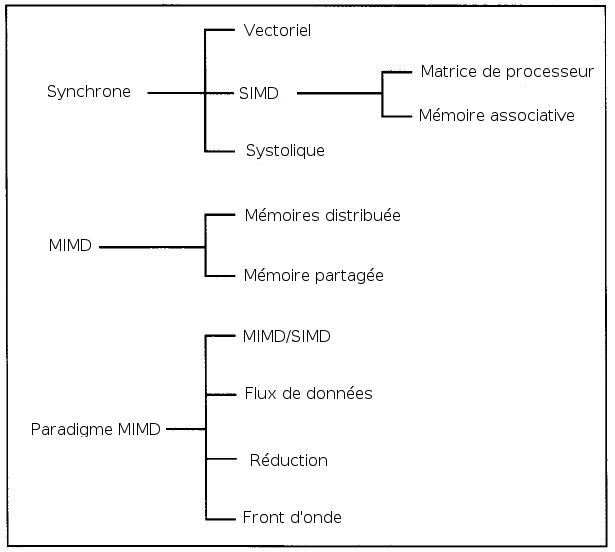
\includegraphics[width=16.272cm,height=14.605cm]{Biblio_PCmax_Rendu_Taxonomie_Duncan.jpg}
\par}
{\centering
Taxonomie de haut niveau de l'architecture de l'informatique parallèle.
\par}
\lp{Mettre le titre avec caption, environnement figure}

\bigskip

\begin{itemize}
\item Les architecture synchrones.
  Ces architectures coordonnent les opérations concurrentes via une
  horloge globale et un contrôleur de programmes.(i) Les processeurs
  vectoriels permettent un traitement parallèle en envoyant
  séquentiellement des éléments vectoriels dans des pipelines d'unités
  de traitements mis en cascades.(ii) Les machines systoliques,
  pulsent le déplacement des données entre mémoire et réseau de
  processeurs, à un rythme soutenu.
  (iii) Les SIMD, emploient une unité de contrôle centrale, et de
  multiples processeurs.
  On distingue les SIMD à matrice de processeurs, (calibrés pour le
  calcul scientifique à grande échelle, le traitement d'images) où on
  retrouve les GPU, et les SIMD à mémoire associative
  (particulièrement adaptés pour le traitement de bases de données, le
  suivi, la surveillance).
\item Les architectures asynchrones, de type MIMD, emploient plusieurs
  processeurs pour exécuter des flux d'instructions indépendant, en
  utilisant des données locales.
  On distingue, d'une part, les MIMD à mémoire distribuée.
  Les processeurs ont leur propre mémoire, et le partage d'information
  s'opère uniquement par échange de messages.
  On rencontre dans ce type d'architecture, les grappes, les MPP
  (Massive Parallel Processing) et les COW (Cluster Of Workstations).
  Et d'autre part les MIMD à mémoire partagées, telles que les
  machines muti-processeurs, ou les processeurs multi-c\oe{}urs.
  \lp{Dire que c'est le contexte de ton travail ?}
\item Les architectures mixtes, ou basées sur le paradigme MIMS.
  (i) Les hybrides MIMS/SIMS sont des architectures MIMD pilotées de
  la même façon que les SIMD.
  (ii) Les architectures à flots de données sont pilotées par les
  dépendances des données elles-mêmes.
  (iii) Les architectures à réductions sont utilisées pour les langages
  de programmation fonctionnels, dont les expressions sont récursives.
  (iv) Les architectures Front d'onde (wavefront) sont un mélange des
  architectures à flots de données et des architectures systoliques.

\end{itemize}

%\lp{la classification de Flynn date un peu... Peut-être faut-il 
% trouver qlqchose de plus récent}
%\tdi{FCO: ok, fait}


Les premières machines parallèles étaient des réseaux
d'ordinateurs, et des machines vectorielles (faiblement
parallèles, très coûteuses), telles que l'IBM 360, les
Cray1. 
De nos jours, les super-ordinateurs ont un nombre de c\oe{}urs de l'ordre de plusieurs millions, et leur performances de calculs s'expriment 
en centaines de petaFLOP. Les 500 super-ordinateurs les plus puissants 
sont recensés par le site www.top500.org. 
Le Supercomputer Fugaku (Fujitsu), du Centre pour la science 
des ordinateurs de RIKEN au Japon (figure \ref{fig:Fugaku}), 
vient de détrôner depuis juin 2020 le Summit (IBM) 
de l’Oak Ridge National Laboratory aux États-Unis.

%	\lp{Ce n'est pas si simple. On continue de faire, et d'utiliser
%  	  des machines vectorielles, les GPU sont aussi du SIMD...}
%	\tdi{FCO: ok, fait}
\bigskip

\begin{figure}
\centering
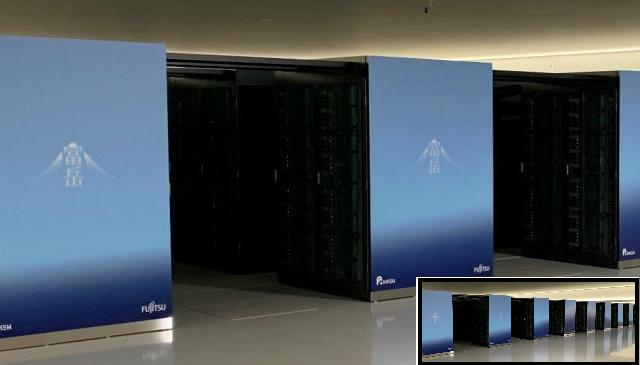
\includegraphics[width=11.29cm,height=6.44cm]{Biblio_PCmax_Rendu_Fugaku.jpg}
\caption{Le Supercomputer Fugaku (Fujitsu), 
  Il compte 7,630,848 c\oe{}urs basés sur des processeurs ARM A64FX
  48C cadencés à 2.2GHz, 5,087,232 GB de ram, pour une performance de 442 PFLOPS. 
  Il fonctionne sous Red Hat Entreprise Linux (RHEL).}
\label{fig:Fugaku}
\end{figure}

% \lp{pense à compléter cette partie avec des infos sur des
%  machines actuelles. voir top500.org dont il serait peut-être plus
%  judicieux de citer les infos: puissance des plus gros ordinateurs,
%  nombre de proc, cores, etc. Parler peut-être aussi des clouds ? Des
%  applications ? Pour intro}
% \tdi{FCO: ok, fait}
On peut définir une machine parallèle comme un ensemble de processeurs
capables de coopérer et de communiquer dans le but de résoudre un
problème plus rapidement.
Les clusters, ou grappes (MIMD à mémoire distribuée), sont
principalement homogènes.
Avec internet, il devient possible d'interconnecter des ordinateurs,
voire des grappes, et de créer ainsi, à l'instar d'un réseau de
distribution d'électricité, un système distribué grande échelle,
appelé grid, ou grille.
Une grille relie des ordinateurs (PC, portable,
Superordinateur, cluster), des systèmes de bases de données
(e.g base du génome humain, atlas astronomique de Strasbourg), et dans
certains cas, des instruments spéciaux 
(e.g le radio-télescope d'Arecibo). 
Les applications liées aux grilles sont diverses.
On peut citer le web (la première grille), le \emph{Cloud
  computing}, les web-services, les réseaux \emph{peer-to-peer},
l'\emph{internet computing}, comme le projet SETI
(www.boinc-af.org/setihome.html).
Ce projet consiste à rechercher des preuves possibles de transmissions
radio provenant d'intelligences, autres que terrestres, à l'aide de
données fournies par un radiotélescope.
Le "serveur", distribue, une portion d'échantillons radio à traiter
aux clients volontaires (logiciel client installé sur un PC), pour
ensuite recouper les résultats.
En tout, ce sont cinq millions de participants, qui ont accumulé deux
millions d'années de calculs depuis la création du projet en 1999.
Se pose alors le problème de l'attribution des tâches aux postes
clients, un problème d'ordonnancement.


\subsection{Ordonnancement}

Sur une machine non parallèle, les tâches sont exécutées
séquentiellement, les unes après les autres.
Certaines tâches, ou jobs peuvent demander plus de temps que d'autres
pour être entièrement traitées.
Lorsque plusieurs ressources (processeurs, machines, c\oe{}urs) sont
disponibles, ou que des jobs a exécuter ne sont pas indépendants (même
traités sur un seul processeur), se pose alors, un problème
d'ordonnancement.
Celui-ci consiste à organiser, dans le temps, les jobs à exécuter, en
les affectant à une ressource donnée, de manière à satisfaire un
certain nombre de contraintes, tout en optimisant un ou des objectifs.
L'ordonnancement fait partie de la catégorie des problèmes
d'optimisation combinatoire, et est un champ de la recherche
opérationnelle, très actif depuis plus d'un siècle.

Les problèmes qui s'y rattachent sont très variés.
Premièrement, la nature des machines parallèles doit être considérée.
Celles-ci peuvent être:
\begin{description}
\item[identiques] le même temps de traitement sera nécessaire, d'une
  machine à l'autre;
\item[uniformes] un quotient de vitesse $q_i$ propre à une machine est à
  appliquer pour chaque tâche affectée à cette machine pour déterminer
  le temps de traitement nécessaire;
\item[indépendantes] les temps de traitements des tâches sont ni
  uniformes ni proportionnels d'une machine à l'autre.
\end{description}
Ensuite, des contraintes peuvent affecter les jobs eux-mêmes.
Dans le cas d'un problème préemptif, les tâches peuvent être
interrompues, et reprises ultérieurement.
Il est possible que les jobs soient indépendants, ou au contraire,
être liées par des relations de précédence.
Ces jobs ne sont disponibles qu'à partir d'une certaine date.
Ou encore, être de durée égale, ou tous de durée différente.

Pour finir, l'objectif de
l'ordonnancement est d'optimiser un
critère. Par exemple, minimiser la somme des dates de fin, la somme
des retards, le nombre de tâches en retard, ou simplement, le retard
total. Mais le plus habituel, est de chercher à minimiser le temps
total de traitement de tous les jobs, i.e minimiser le makespan.
\lp{Ajouter: ``noté $C_{\max}$'' sinon ce n'est pas défini.}

% \lp{définir la notation de Graham à la fin de cette partie
%   puisque tout y est déjà dit.}
% \tdi{FCO: ok, fait}

Ces diverses possibilités définissent divers problèmes
d'ordonnancements différents, recensés et classifiés
\ par Graham \emph{et al.} \citep{graham1979optimization}, qui introduit la notation trois-champs $\alpha
${\textbar}$\beta ${\textbar}$\gamma $ .

\bigskip

Le problème \problemGrahamP se définit alors ainsi:
\lp{Ajouter: ``Dans cette classification, ...''}

\begin{itemize}

% -------------------------------------------------------
% ALPHA P Type de machines
% -------------------------------------------------------
\item $\alpha = \alpha_1 \alpha_2$, détermine l'environnement
  machines.
  $\alpha P$:
  \lp{Je ne comprends pas pourquoi $\alpha$ ? $\alpha=P$?}
  les machines sont parallèles et identiques: un job,
  une tâche prendra le même temps de traitement qu'il soit exécuté sur
  une machine ou une autre.
  Le nombre de machines ($m$) est variable.

% -------------------------------------------------------
% BETA Contraintes
% -------------------------------------------------------
\item
  $\beta \subset \{ \beta_1, \beta_2, \beta_3, \beta_4, \beta_5,
  \beta_6\}$, détermine les caractéristiques des jobs, ou des
  tâches. Ici $\beta$ est vide, ce qui signifie que la préemption
  n'est pas autorisée (les jobs doivent être exécutés d'une traite,
  sans interruption ni coupure) et qu'il n'y a pas de relation entre
  les jobs (ils sont indépendants).

% -------------------------------------------------------
% GEMEL Optimisation
% -------------------------------------------------------
\item $\gamma $ détermine le critère à optimiser.
  $\gamma C_{\max}$:
\lp{Idem $\gamma = C_{\max}$?}
  on cherche à optimiser le makespan,
i.e.\ le temps de traitement total.

\end{itemize}
\bigskip


\subsection{Énoncé du problème GrahamP\problemGrahamP}


\begin{definition}{\problemGrahamP}

  \problemGrahamP consiste à planifier un ensemble
  $J = \{j_1,j_2,\ldots,j_n)$ de $n$ jobs simultanés, pour être
  traités par $m$ machines identiques et parallèles.  \lp{Ce sont des
    machines identiques mais non parallèles. Le fait qu'il y en ait
    plusieurs fait que c'est un problème de parallélisme} Chaque job,
  qui requière une opération, peut être traité par une des $m$
  machines.  Le temps de traitement de chaque job $p_i$ (avec
  $i \in \mathbb{N}$) est connu à l'avance.  Un job commencé est
  complété sans interruption.  Les jobs, indépendants, sont exécutés
  par une seule machine, et une machine ne peut traiter qu'un seul job
  à la fois.
  \lp{Dire jobs séquentiels et non parallèles?}

la notation:
\begin{itemize}
\item \problemGrahamP ou \problemGrahamPm précise que le nombre de
  machines $m$ est fixe, et est connu à l'avance dans l'instance du
  problème, mais reste une variable.
  \lp{Pour moi $P_m$ signifie que la solution donnée ne l'est que pour
    $m$ machines. Si la solution l'est quelquesoit le nombre de
    machines, le nombre de machines étant fixe mais une donnée du
    problème alors c'est \problemGrahamP}
\item \problemGrahamPII fixe le nombre de machines parallèles.
  ici, deux.
\end{itemize}

\end{definition}


\lp{on peut recontextualiser l'intérêt du problème. A l'heure
  actuelle, bon nombre de centres de calcul ont un parc
  assez homogène. De même les clouds offrent des instances de VM, ce
  qui permet d'avoir un environnement d'exec homogène }

\lp{faire un dessin illustratif ?}


% \lp{dire que la difficulté repose uniquement sur le regourpement
%   des jobs sur une machine puisque les machines sont identiques}
% \todo{FCO: Rechercher exemples}
\subsection{Notations}
Chaque document utilise sa propre notation, mais les notions sont les mêmes.
Soient les données du problème:

\begin{itemize}
% -------------------------------------------------------
% ENSEMBLE DES JOBS J (itérateur j)
% -------------------------------------------------------
\item J, un ensemble de $n$ jobs (ou tâches) 
	$J = \{J_1, J_2, ..., J_n\}$ 
dont chaque job $J_j$ a un temps de traitement connu 
$P_j \in P = \{P_1, P_2, ..., P_n\}$
\lp{Je ne pense pas qu'il soit utile (nous ne le faisons pas en
  général) de définir un ensemble de temps d'exécution.}
\lp{Il serait mieux de garder les majuscules pour les ensembles et les
  minuscules pour les éléments. Mais peut-être le travail est trop
  conséquant pour valoir le coup ?}

% -------------------------------------------------------
% ENSEMBLE DES MACHINES M (itérateur i)
% -------------------------------------------------------
\item M, un ensemble de $m$ machines parallèles identiques 
	$M = \{M_1, M_2, \ldots, M_m\}$

%  \lp{au besoin définir $M = \{ m_1, m_2, \ldots, m_m \}$ mais du
%  coup il faut choiir à quoi sert le $m$}

%	\tdi{FCO: M (majuscule) est l'ensemble des m machines parallèles
%  	identiques.
%   $m_i$ est une machine de M, avec $1<= i<= m$, il y a double emploi
%  	entre m la machine et m le nombre de machines, mais m en tant que
% 	nombre est utilisé (aussi) dans \problemGrahamPm.
%	Donc j'ai tout mis en majuscule lorsqu'il s'agit d'une entité,
%   (machine, job, temps) et en minuscule, pour les nombres}

% -------------------------------------------------------
% RESULTAT DE L'ALGORITHME A
% -------------------------------------------------------
\item $C_m^A(J)$ Le résultat (makespan) de l'ordonnancement 
	d'un ensemble $J$ de jobs, 
	sur m machines parallèles, identiques, 
	obtenu par l'algorithme $A$.
%  \lp{à quoi sert $j$ ici ?}
%  \tdi{FCO  ok, fait : C'était une erreur de frappe ...
%	le copier/coller qui va avec}

% -------------------------------------------------------
% RESULTAT OPTIMAL
% -------------------------------------------------------
\item $C_m^\star(J)$ Le makespan optimal, idéal, de l'ordonnancement 
	d'un ensemble $J$ de jobs, 
	sur $m$ machines parallèles identiques.
%  \lp{idem}
%	\tdi{FCO: ok, fait}
% -------------------------------------------------------
% RATIO OBTENU/OPTIMAL
% -------------------------------------------------------
\item $\Gamma(A)=\dfrac{C_m^A(J)}{C_m^\star(J)}$ 
	Le ratio d'approximation atteint par l'algorithme $A$ au pire cas.

\lp{Définir $C^*$}
%  \tdi{FCO: ok, fait}
\end{itemize}



\subsection{Problématique}

Comme l'ont démontré Garey et Johnson,
\problemGrahamPII est un
problème NP-Difficile \citep{garey1978strong}, et
\problemGrahamP est un problème NP-Difficile
au sens fort \citep{garey1982computers} \lp{Pour plus de 3 machines ?}.
Cependant, \problemGrahamP devient un problème NP-Difficile, du moment
que le nombre de machines est fixé \cite{chen1999potts}, comme l'a
montré Rothkopf \cite{rothkopf1966scheduling}, qui a présenté un
algorithme de programmation dynamique.

Donner la solution optimale à un problème d'ordonnancement (dans notre
cas \problemGrahamP) n'est pas réaliste.
Même pour un problème de taille modeste\lp{Tout dépend du niveau
  auquel tu places la modestie, donc peut-relativisé. Perso je n'ai
  aucune idée de la taille limite}, la résolution de celui-ci
demanderait un temps excessif et donc rédhibitoire.

Comme les machines sont identiques, et travaillent à la même vitesse,
la difficulté, repose uniquement sur le regroupement des jobs et choix
d'affectation d'une machine pour chaque regroupement.  \lp{Justement
  non, il n'y a plus de choix d'affectation à faire une fois les
  regroupements fait puisque toutes les machines sont les mêmes cela
  ne change rien qu'on en prenne l'une ou l'autre. Par contre on peut
  aussi dire qu'on affecte les tâches à des machines, pour définir
  implicitement les regroupements}

La résolution du problème d'ordonnancement va reposer sur des méthodes
d'approche, qui consistent à calculer en
temps polynomial, une solution ``assez'' proche de la valeur optimale.
% \todo{LP: approximation?}\todo{FCO: c'est bien le bon terme}

\begin{theoreme}
Toutes les solutions ont une borne minimale \\
 $= \max \{ \max_j\{P_j\}, \sum_{j=1}^{n} \dfrac{P_j}{m} \}$
\label{theoreme:borneMini}
\end{theoreme}
\lp{Si on ne le démontre pas je pense que ça n'est pas la peine de
  mettre cette borne sous la forme d'un théorème. Par contre, cela
  pourrait avoir du sens d'expliquer informellement cette borne}

Dans la littérature, l'étude d'ordonnancement est très riche et
abondante.
Le but étant d'améliorer le temps de calcul, et d'approcher le
résultat optimal.
L'existence d'une solution qui résout le problème \lp{... de manière
  optimale...} n'étant pas pensable, à moins que $P = NP$, \lp{les
  solutions proposées dans la littérature sont des heuristisques ou
  des approximations}. 


\section{Heuristiques}

%	\lp{définir heuristic ?}
%	\tdi{FCO: ok, fait}

Le but d'une heuristique (du grec \emph{heuriskein}: trouver) est
de trouver une solution respectant les contraintes du problème et de
bonne qualité selon le critère d'optimisation considéré.
La solution ne sera pas forcément optimale, mais une heuristique
efficace tente de trouver une solution de bonne qualité, suivant le
temps de résolution imparti.
E.g.\ pour le voyageur de commerce, on peut choisir l'heuristique ``du
plus proche voisin''.
On choisit la ville la plus proche de la ville courante, jusqu'à avoir
visité toutes les villes.
Cette heuristique est simple, mais donne un très mauvais résultat
\lp{Je relativiserais le très, cela dépend du problème}.

%Les heuristiques présentent plusieurs avantages. Leur complexité est
%réduite\lp{ça dépend de leur conception}, et obtiennent de bonne
%performances\lp{ça dépend aussi, je suis capable de faire des
%heuristiques non performantes}.
Ces algorithmes donnent des résultats, dont la borne maximale, au pire des cas  n'est pas maîtrisée : 
une étude du comportement est nécessaire pour définir cette borne
maximale.\lp{Elle n'existe pas parfois. Dans ce cas, l'étude de comportement (ou
  simulation) permet d'avoir des indications générales sur le comportement}
% \lcc{revoir notation et phrase}
% \fco{ok, fait.}
% $C_m^A(J)_{maximal}$

Les heuristiques représentent la plus grande partie des recherches concernant le problème
d'ordonnancement.

%même si leurs performances, au pire cas, ne sont pas\todo{LP: ??}\todo{FCO : pour dire %que, contrairement aux PTAS, le ratio n\ap est pas maîtrisé} garanties.
%Sont abordées ici les heuristiques les plus présentes dans la littérature.

% \lp{on a aussi une borne min qui est le max entre la plus grande
%   des tâches et sum(pi)/m}
% \fco{FCO: ok, fait: Cette borne est une caractéristique du problème.}
\subsection{LS (List Scheduling)}
% '

L'idée d'une LS est de stocker l'ensemble des jobs dans celle-ci,
les trier dans un ordre \lp{on parle souvent de prioritté} particulier,
avant de les affecter à une machine selon des règles définies.
Le premier job de la liste étant affecté à la première machine disponible.

%	\lp{un algorithme de liste affecte aussi un job, le premier de la
%	liste, à la première machine prête}
%	\tdi{FCO: ok, fait}
%\bigskip
% -------------------------------------------------------
% LPT Rule
% -------------------------------------------------------
\subsubsection{LPT rule} % (Graham \emph{et al.}, 1969)}

% Présentaion
% ---------------------
Graham propose \emph{Longest Processing Time (LPT) rule} \cite{graham1969bounds}.

\bigskip
% Algorithme
% ---------------------
\begin{algorithm}[H]
\DontPrintSemicolon 
\KwData{instance de \problemGrahamP, avec $m$ machines, $n$ jobs et leur temps d'exécution}
%\Begin{ %inutile ici et rajoute un nuero de ligne

\BlankLine % Petit espace
Trier les jobs de l'ensemble $J$ dans l'ordre décroissant de leur temps
d'exécution et ré-indexer l'ensemble de telle manière à obtenir:
$P_1 \geq P_2 \geq \ldots \geq P_n$

\BlankLine % Petit espace
Parcourir la liste et affecter chaque job à la machine la moins
chargée à ce moment là.
% }
\caption{LPT Rule\label{algo:LPT}}
\end{algorithm}

\bigskip
% Exemple
% ---------------------

\begin{figure}
{\centering
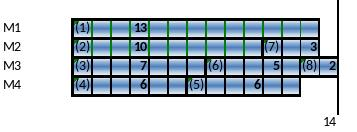
\includegraphics[width=8.334cm,height=4.034cm]{Biblio_PCmax_Rendu_exLPT1.jpg}
\caption{Ordonnancement obtenu avec LPT.}
\label{ex:LPTExempleAlgo}
\par}
\end{figure}

\begin{example}
Soit $P=\{13,10,7,6,6,5,3,2\}$, l'ensemble des $P_j$ déjà triés dans
l'ordre décroissant à appliquer sur 4 machines parallèles identiques:

Nous obtenons $C_4^{LPT}(J)=14$ (figure \ref{ex:LPTExempleAlgo}).
\end{example}

% Complexité
% -------------------------------------------------------
\begin{theoreme}
\begin{flushleft}
\begin{tabular}{|p{8cm}p{6cm}|}
% TITRES (pas de titre)
\hline
% Ligne blanche
& \\
% Ligne Complexité en temps
Le tri puis l'affectation coûtent en temps:& $O(n \log n + n \log m)$
\\	% pas de ligne \hline
% RATIO
Le ratio d'approximation:	&	$\Gamma(LPT)\leq \dfrac{4}{3} - \dfrac{1}{3m}$
\\
% Ligne blanche
& \\
\hline
\end{tabular}
%pas de legende
\end{flushleft}
\end{theoreme}

% \lcc{précision complexité en temps}
% \tdi{FCO: ok, fait}

% -------------------------------------------------------
% LPT-REV
% -------------------------------------------------------
\subsubsection{LPT-Rev} % (Croce \emph{et al.}, 2018)}

% Présentaion
% ---------------------
Le ratio d'approximation obtenu par LPT (algorithme \ref{algo:LPT})
$(\Gamma(LPT)\leq \dfrac{4}{3} - \dfrac{1}{3m})$ est une borne
supérieure que cet algorithme peut atteindre, mais qu'il ne dépassera
jamais.
Chaque utilisation de LPT produira un résultat dont le ratio $\Gamma$
oscillera entre 1 et $\dfrac{4}{3} - \dfrac{1}{3m}$.
\bigskip

% figures pour l'explication
% ---------------------
\begin{figure}
{\centering}
% Exemple à gauche
	\begin{subfigure}[b]{0.45\linewidth}
    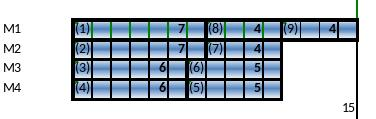
\includegraphics[width=\linewidth]
    {Biblio_PCmax_Rendu_exLPT_Rev1.jpg}
    \caption{Ordonnancement obtenu avec LPT}
  	\end{subfigure}
\hfill% sinon, en fin de page, et pas sur la même ligne
% Exemple optimal à droite
	\begin{subfigure}[b]{0.45\linewidth}
    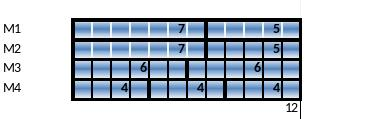
\includegraphics[width=\linewidth]
    {Biblio_PCmax_Rendu_exLPT_Rev2.jpg}
    \caption{Ordonnancement optimal}
  	\end{subfigure}
%CAPTION/FIGURE Complete 
  	\caption{LPT, pire cas}
  	\label{ex:LPTExemplePireCas}
\end{figure}

% Exemple pour l'explication
% ---------------------
\begin{example}
\begin{flushleft}
Exemple de pire cas (figure \ref{ex:LPTExemplePireCas}) de LPT (algorithme \ref{algo:LPT})

Soit $P=\{7,7,6,6,5,5,4,4,4\}$, l'ensemble des $P_j$ déjà triés dans
l'ordre décroissant à appliquer sur 4 machines parallèles identiques:
\bigskip
LPT donne le résultat suivant : $C_m^A(J) = 15$
\bigskip

Un ordonnancement optimal aurait été : $C_4^{\star}(J)=12$

Soit une marge de $\dfrac{15}{12}$

Le ratio d'approximation prévu pour $m=4$:

\[
  \dfrac{4}{3} - \dfrac{1}{3m}=\dfrac{16}{12} - \dfrac{1}{12}=\dfrac{15}{12}
\]

Ce cas représente donc un pire cas pour LPT.
\end{flushleft}
\end{example}

\bigskip

% Definitions
% Machine critique
% Job Critique
% ---------------------
\begin{definition}{Job et machine critique}
Le job critique (noté $J^\prime$) est le job qui détermine le
makespan.

La machine critique est la machine qui exécute le job critique.
\end{definition}

% Introduction
% ALGO LPT-Rev Croce et al.
% ---------------------
Croce \emph{et al.}
\cite{della2018longest}, en examinant le comportement de LPT rule,
notamment au niveau du ratio d'approximation, constatent que celui-ci
peut être réduit selon certaines configurations, ou instances du
problème, et rédigent le théorème suivant:

\begin{theoreme}
  LPT a un rapport d'approximation non supérieur à\\
  $\dfrac{4}{3} - \dfrac{1}{3(m-1)}$ pour $m \geq 3$ et $n \neq 2m+1$.
\end{theoreme}

\bigskip
LPT atteint la limite de Graham $\dfrac{4}{3} - \dfrac{1}{3m}$ pour
$m \geq 2$ et uniquement dans le cas où $n=2m+1$, et la machine
critique traite 3 jobs, tandis que les autres en traitent 2.


% \lcc{Les définitions à l'extérieur des théorèmes.}
% \fco{ok, fait}



Le rapport $\dfrac{4}{3} - \dfrac{1}{3(m-1)}$ est inférieur au
ratio $\dfrac{4}{3} - \dfrac{1}{3m}$ (quel que soit le nombre de
machines)

\bigskip

\textbf{NB}
\lp{Tout ceci est déjà dit}
L'exemple précédant (pire cas) a les caractéristiques suivantes:
\begin{itemize}
	\item nombre de job $n=2m+1$.
	\item la machine critique exécute 3 jobs.
	\item les autres exécutent 2 jobs.
	\item un rapport d'approximation de $\dfrac{4}{3} - \dfrac{1}{3m}$
\end{itemize}

\bigskip

Une modification à l'algorithme LPT rule est apportée afin de placer
le problème \problemGrahamP toujours dans une instance où le ratio
d'approximation est $\leq \dfrac{4}{3} - \dfrac{1}{3(m-1)}$.
Cette modification consiste à planifier en premier, le job critique
sur une machine M1.

\bigskip
% \todo{FCO: Algos tous en anglais ou tous en français}

% Algorithme
% ---------------------
\begin{algorithm}[H]
\DontPrintSemicolon
\KwData{instance de \problemGrahamP, avec m machines, n jobs}
%\Begin{ %inutile ici et rajoute un nuero de ligne

Appliquer LPT ce qui donne un ordonnancement avec 
un makespan $z_1$ et $k-1$ jobs sur la machine critique avant le job $J^\prime$
\BlankLine % Petit espace

Appliquer $LPT^\prime = LPT(J^\prime)$ 
ce qui donne une solution avec un makespan $z_2$
\BlankLine % Petit espace

\Si{  $m=2$ } 
{
Appliquer $LPT''=LPT([(J^\prime - k + 1), ...
, J^\prime])$ 
ce qui donne une solution avec un makespan $z_3$ \\
\Return $\min(z_1,z_2,z_3)$
}
\Sinon
{
\Return $\min(z_1,z_2)$

}
\caption{LPT-Rev\label{algo:LPTRev}}
\end{algorithm}


\bigskip

% Complexité
% -------------------------------------------------------
\begin{theoreme}
\begin{flushleft}
\begin{tabular}{|p{8cm}p{6cm}|}
% TITRES (pas de titre)
\hline
\\
% Ligne blanche
Complexité en temps:	& $O(n \cdot log (n))$
\\
% RATIO
Ratio d'approximation:	&	$\Gamma(LPT-REV)\leq \dfrac{4}{3} - \dfrac{1}{3(m-1)}$
\\
% Ligne blanche
& \\
\hline
\end{tabular}
%pas de legende
\end{flushleft}
\end{theoreme}

\subsubsection{D'autres algorithmes}
Il existe d'autres propositions basée LS, telles que 
AP de mokotoff \emph{et al.} \cite{mokotoff2004exact}
\lp{Dire en 2 mots ce qu'ils font ?}
 


\subsection{Bin-Packing}

Le problème Bin-packing, est semblable au problème \problemGrahamP.
Il consiste à ranger des objets de taille différentes, dans des bacs
identiques, tout en minimisant leur nombre.

L'ensemble des n jobs $J = \{J_1, J_2, \ldots, J_n\}$, et de leurs temps de
traitement $P_j \in P = \{P_1, P_2, ..., P_n\}$, peuvent être vus
respectivement comme:
\begin{itemize}
\item un ensemble d'objets $T_j \in T = \{T_1, T_2, ..., T_n\}$
\item leur taille $L(T_j)$ avec $1 \le j \le n$
\end{itemize}
Une taille maximale $C$ des bacs (ou boites) est donnée.
\bigskip

\begin{definition}{Packing}
  Un packing, est une partition $P<P_1, P_2, ..., P_m>$ tel que
  $L(P_i) \leq C$ avec $1 \leq i\leq m$.
  Le but est de placer les objets $T_j$ dans des bacs $P_i$ de taille
  $C$, de manière à minimiser le nombre de bacs $m$.
\end{definition}

le problème Bin-packing est NP-Complet \cite{Johnson1974WorstCasePB}.

L'idée est d'utiliser le problème Bin-Packing à l'envers, pour
approcher une solution au problème d'ordonnancement.

% \lp{petite remarque sur la complexité du problème ?}
% \tdi{FCO: ok, fait}

% -------------------------------------------------------
% MULTIFIT
% -------------------------------------------------------
\subsubsection{Multifit}

% Présentaion
% ---------------------
Coffman \emph{et al.} \cite{coffman1978application} se sont
intéressés à l'algorithme FFD (First Fit Decreasing), un outil de
résolution du problème de Bin-Packing, pour l'adapter au problème
\problemGrahamP.
$FFD(T,C)$ renvoie le nombre de bacs de taille C non vides
nécessaires, et l'arrangement correspondant de l'ensemble $T$ d'objets.

\bigskip
% Principe de l'algorithme
% ---------------------
Soit $T_m^\star = \min\{C:FFD(T,C) \leq m\}$ la plus petite valeur de
$C$ (taille des bacs) qui permet à $T$ d'être pacqué dans $m$ (ou moins)
bacs.

\bigskip


L'idée de MULTIFIT est donc de proposer une valeur pour $C$, faire
tourner $FFD(T,C) $, et réduire à chaque itération cette valeur de $C$
jusqu'à ce que le nombre $m$ de bacs renvoyé par $FFD(T,C) $, alors
devenu insuffisant, augmente à $m+1$ (figure \ref{ex:MULTIFITExempleAlgo}).
Cette valeur charnière de $C$ est $T_m^\star$, qui correspond au
makespan minimum recherché, de l'ordonnancement de l'ensemble $T$ de
jobs sur $m$ machines identiques parallèles.
La difficulté, est de proposer une première valeur de $C$ pas trop
éloignée de la valeur recherchée, afin de réduire au maximum le nombre
d'itérations.
% \lp{deux mots pour dire comment est implémentée la recherche}
% \tdi{FCO: ok, fait}

La méthode utilisée est une recherche dichotomique.
Après avoir défini les bornes supérieure
$C_u = \max\{\dfrac{2}{m} \cdot L(T), \max_i\{L(T_i)\} \}$ et
inférieure $C_l = \max\{\dfrac{2}{m} \cdot L(T), \max_i\{L(T_i)\} \}$
de départ, FFD est exécuté avec le milieu $C_d = \frac{C_u + C_l}{2}$.
si $FFD(T,C_d)\le m$ alors la nouvelle fourchette de recherche devient
$C_u = C_d$ et $C_l$, sinon (si $FFD(T,C_d)> m$) alors la nouvelle
fourchette devient $C_u$ et $C_l = C_d$.
Un nombre d'itérations $k$ et donné à l'exécution de MULTIFIT, estimé
en fonction de la taille du problème (n et m).
Mais même pour un problèmes de grande taille, le résultat ne change
plus après $7$ itérations.
Il est donc inutile d'utiliser $k>7$.

\begin{figure}
\centering{
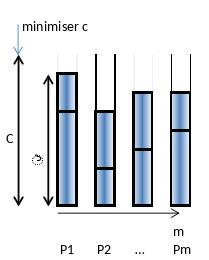
\includegraphics[width=6.5261cm,height=8.12073cm]{Biblio_PCmax_Rendu_exMULTIFIT1.jpg}
\caption{Fonctionnement de FFD et principe de MULTIFIT.}
\label{ex:MULTIFITExempleAlgo}
\par}  	
\end{figure}

\bigskip

% Algorithme
% ---------------------
\begin{algorithm}[H]
\DontPrintSemicolon
\KwData{T un ensemble de jobs

m, un nombre de processeurs

borne supérieure: $Cu[T,m] = \max\{\dfrac{2}{m} \cdot L(T), \max_i\{L(T_i)\} \}$

borne inférieure: $Cl[T,m] = \max\{\dfrac{1}{m} \cdot L(T), \max_i\{L(T_i)\} \}$

k un nombre d'itérations
}

\BlankLine % Petit espace
La recherche de $T_m^\star$ s'effectue par dichotomie sur k itérations

\BlankLine % Petit espace
Après les k itérations, MULTIFIT \Return {$Cu(k)$} \\
\tcp{qui correspond à la plus petite valeur de $C$ 
pour laquelle $FFD[T,C] \leq m$}

\caption{MULTIFIT\label{algo:MULTIFIT}}
\end{algorithm}
% \lp{$k$ fixé ? ou seuil entre deux iter ?}
% \tdi{FCO: ok, fait}

\bigskip

% Complexité
% -------------------------------------------------------
\begin{theoreme}
\begin{flushleft}
\begin{tabular}{|p{8cm}p{6cm}|}
% TITRES (pas de titre)
\hline
% Ligne blanche
& \\
% Ligne Complexité
Tri puis k FFD coûtent en temps: & $O(n \log n + kn \log m)$
\\	% pas de ligne \hline
% Ligne blanche
& \\
% RATIO
Ratio \cite{lee1988multiprocessor}:& $\Gamma(MULTIFIT) \leq 1,220 + 2^{-k}$
\\
% Ligne blanche
& \\
\hline
\end{tabular}
%pas de legende
\end{flushleft}
avec k le nombre d'itérations pour la recherche dichotomique.
\end{theoreme}

Généralement, MULTIFIT donne des résultats très satisfaisant avec $k = 7$


% -------------------------------------------------------
% COMBINE
% -------------------------------------------------------
\subsubsection{Combine}

% Présentaion
% ---------------------
Lee \emph{et al.}, \cite{lee1988multiprocessor} ont l'idée
d'utiliser LPT (algorithme \ref{algo:LPT}) pour réduire les bornes de départ
et ainsi optimiser MULTIFIT (algorithme \ref{algo:MULTIFIT}) dans un algorithme nommé COMBINE.

% \lp{développer/préciser un peu}
% \tdi{FCO: ok, fait}
\bigskip
soient
\begin{align*}
&\textnormal{la moyenne des poids des jobs par processeur} &A &= \sum_{i=1}^{n}(\dfrac{P_i}{m})\\
&et &M &= C_m^{lpt}(J) \\
& &M^\star &= C_m^\star(J)
\end{align*}

COMBINE, améliore certains points de l'algorithme MULTIFIT en se basant
sur les principes suivants:
\begin{itemize}
\item Le résultat $M$ obtenu par LPT, est forcément supérieur ou égal
  à $M^\star$, soit $M \ge M^\star$.
  COMBINE utilise donc $M = C_m^{lpt}(J)$ comme borne supérieure $C_u$
  de départ pour la recherche dichotomique utilisée par MULTIFIT.
  celle-ci est beaucoup plus proche du résultat optimal que la borne
  supérieure de départ $2\cdot A$ utilisée à l'origine par MULTIFIT.
\item Si Le résultat $M$ obtenu par LPT est tel que
  $M \geq 1,5\cdot A$ alors $M=M^\star$.
  Il n'est donc pas nécessaire de poursuivre la recherche.\lp{Je ne
    comprends pas pourquoi}
\item Au lieu de prédéterminer un nombre d'itérations, COMBINE utilise
  une condition d'arrêt de la recherche dichotomique, en fonction de
  l'écart entre les deux bornes.
  COMBINE stoppe la recherche dès que $C_u - C_l \le \alpha \cdot A$.
  Les tests de COMBINE ont été effectués avec $\alpha = 0,005$
\end{itemize}


\bigskip
% \todo{FCO: Algo tout en anglais ou français}
% Algorithme
% ---------------------
\begin{algorithm}[H]
\DontPrintSemicolon
\KwData{instance de \problemGrahamP, avec m machines, n jobs, et un coefficient $\alpha (0,005)$ }

A = $\sum_{i=1}^{n}(\dfrac{P_i}{m})$

\BlankLine % Petit espace

M $\leftarrow C_m^{lpt}(J)$

\BlankLine % Petit espace

\Si {$M \geq 1,5 \cdot A$}
 {
 	$M^\star = M$ \;
 }
\Sinon
 {
	$C_u \leftarrow M$					\;
	$C_l \leftarrow \max \{(\dfrac{M}{\dfrac{4}{3}-\dfrac{1}{3 \cdot m}}),P1,1 \}$	\;
	\Tq {$C_u - C_l > \alpha \cdot A$}
	 {
	 appliquer MULTIFIT \;

	 } \tcp{on arrête lorsque $C_u - C_l \leq \alpha \cdot A$}
 }

\caption{COMBINE\label{algo:COMBINE}}

\end{algorithm}


\bigskip

% Complexité
% -------------------------------------------------------
\begin{theoreme}
\begin{flushleft}
\begin{tabular}{|p{8cm}p{6cm}|}
% TITRES (pas de titre)
\hline
% Ligne blanche
& \\
% Ligne Complexité
Complexité en temps: & $O(n \log n + kn \log m)$
\\	% pas de ligne \hline
% Ligne blanche
& \\
% RATIO
Ratio \cite{gupta2001listfit}: & $\Gamma(COMBINE) \leq \dfrac{13}{12} + 2^{-k}$
\\
% Ligne blanche
& \\
\hline
\end{tabular}
%pas de legende
\end{flushleft}
avec k le nombre d'itérations pour la recherche dichotomique.
\end{theoreme}

Concernant la complexité, pour atteindre
$C_u - C_l \leq \alpha \cdot A$, généralement, 6 itérations suffisent
($k=6$).
Mais COMBINE a déjà exécuté une fois LPT (donc $k=7$).


% -------------------------------------------------------
% LISTFIT
% -------------------------------------------------------
\subsubsection{Listfit}

% Présentaion
% ---------------------
Gupta \emph{et al.}, \cite{gupta2001listfit}, ont aussi l'idée
d'utiliser MULTIFIT (algorithme \ref{algo:MULTIFIT}), afin de réaliser l'algorithme
LISTFIT.

Celui-ci sépare la liste des travaux en 2 sous-listes, traitée soit
dans un ordre LPT (Longest Time Processing), soit dans un ordre SPT
(Shortest Time Processing).
Puis LISTFIT combine ces 2 sous-listes en appliquant MULTIFIT à chaque
itération.
\lp{Expliquer l'intérêt, donner une idée intuitive}

\bigskip
% \todo{FCO: enlever les goto}
% \tdi{FCO: ok, fait}
% Algorithme
% ---------------------
\begin{algorithm}[H]
\DontPrintSemicolon
\KwData{n, m, $p_j$ for $j=1, \ldots, n$}

%STEP 1
Soient $r=1$, $q=0$, $C_{\max}=C_{\max}(LPT)$ : le makespan obtenu par LPT

\BlankLine % Petit espace
\Tq {$q<2$}
{
	$t = 0$ \\
	$q = q + 1$ \\
	\Tq {t < 2}
	{
		$ t = t + 1$
	
		Soient $\Phi = \varnothing$, A = $\{1,...,n\}$, $B = \varnothing$\\\lp{$\Phi = \Phi_q $?}
		Soit  $\omega_r$ la séquence des jobs de la liste des jobs A 
		triés selon l'ordre $\tau$.\\
		\tcp{Si $\tau$ = 1 alors tri en LPT,}
		\tcp{Si $\tau$ = 2 alors tri en SPT.}

		\Tq{$A \neq \varnothing$}
		{


			$\alpha=C_{\max}(MULTIFIT)$: le makespan obtenu via MULTIFIT, 
			avec $\sigma = \Phi_q \cdot \omega_r$
                        ($1^{ère}$ étape de MULTIFIT)
                        
			
			\Si {$C_{\max}>\alpha$} 
				{
				$C_{\max} = \alpha$\\ 
				\Pour {$h=1$ à $m$}
					{$\gamma_h = \pi_h$}
				}
			\Si {$A \neq \varnothing$}
			{
				Retirer le dernier job de $\omega_r$ et le placer dans $B$\\
				Mettre à jour $A$, $\Phi_q$, $\omega_r$.
				$\sigma = \Phi_q \cdot \omega_r$.
			}
		}
	}
}
\tcp{L'ordonnancement où les jobs en $\gamma_h$ sont traités par la machine $h$}
\tcp{est une solution approximative du problème \problemGrahamP }
\tcp{avec un makespan $C_{\max}$.}

\caption{LISTFIT}
\label{algo:LISTFIT}
\end{algorithm}

\bigskip
% Complexité
% -------------------------------------------------------
\begin{theoreme}
\begin{flushleft}
\begin{tabular}{|p{8cm}p{6cm}|}
% TITRES (pas de titre)
\hline
% Ligne blanche
& \\
% Ligne Complexité
Complexité en temps:& $O(n^2 \log(n) + k \cdot n^2 \log(m))$
\\	% pas de ligne \hline
% Ligne blanche
& \\
% RATIO
Ratio \cite{gupta2001listfit} & $\Gamma(LISTFIT) \leq \dfrac{13}{12} + 2^{-k}$
\\
% Ligne blanche
& \\
\hline
\end{tabular}
%pas de legende
\end{flushleft}
avec k le nombre d'itérations pour la recherche dichotomique.
\end{theoreme}

\subsubsection{D'autres algorithmes}
Il existe d'autres propositions telles que :

3-phase de França \emph{et al.} \cite{francca1994composite}

HI-Pcmax de Alvim \emph{et al.} \cite{alvim2004hybrid}\lp{Deux mots explicatifs
  sur ces propositions ?}


\subsection{Approche gloutonne}

% -------------------------------------------------------
% SLACK
% -------------------------------------------------------
\subsubsection{Slack} %(Croce \emph{et al.}, 2018)}

% Présentaion
% ---------------------
Croce \emph{et al.} \cite{della2018longest}, en effectuant la preuve
d'une borne d'approximation pour le
développement de LPT-Rev (algorithme \ref{algo:LPTRev}), ont mis en évidence
l'importance des différences de temps entre les jobs,
ainsi que le regroupement de ceux-ci en sous-ensembles.

\lp{est-ce qu'on sait dire pourquoi ? faire une petite analyse}

notamment pour l'instance suivante:
% * pour ne pas numéroter. Juste besoin d'aligner
\begin{align*}
& \textnormal{Nombre de jobs} &n &=2 \cdot m + 1			\\
& Avec &P_{2 \cdot m + 1} &\geq P_1 - P_m
\end{align*}
Où ils ont planifié d'abord, le job $2 \cdot m + 1$, puis un
sous-ensemble de jobs triés $\{1,...,m\}$ et pour finir un
sous-ensemble de jobs triés $\{m+1,...,2 \cdot m \}$

En résulte l'algorithme suivant: \lp{C'est l'algo le résultat ?}

\bigskip
% Algorithme
% ---------------------
\begin{algorithm}[H]
\DontPrintSemicolon
% \KwData{une instance ...}

%Etape 1
trier la liste des jobs dans l'ordre décroissant des temps nécessaires de traitements

%ETAPE 2
\BlankLine % Petit espace
réindexer les jobs, de manière à obtenir $P_1 \geq P_2 \geq ... \geq P_n$

%ETAPE 3
\BlankLine % Petit espace
Découper l'ensemble obtenu en $\dfrac{n}{m}$ tuples de $m$ jobs (ajout
de jobs "dummy" de taille nulle pour le dernier tuple, si $n$ n'est
pas un multiple de $m$)

%ETAPE 4
\BlankLine % Petit espace
considérer chaque tuple avec la différence de temps (SLACK) entre le
premier job du tuple et le dernier.
\begin{align*}
\{ &\{1, ..., m\} &\{m+1,..., 2 \cdot m\} &... \} \\
   &P_1 - P_m     &P_{m+1}-P_{2 \cdot m}  &...
\end{align*}


%STEP 5
\BlankLine % Petit espace
trier les tuples par ordre décroissant de "Slack" et ainsi former un nouvel ensemble
\tcp{e.g: $\{ \{m+1,..., 2 \cdot m\} \{1, ..., m\}\}$ si $P_{m+1} - P_{2 \cdot m} > P_1 - P_m$.}

%STEP 6
\BlankLine % Petit espace
applique l'ordonnancement (Affectation à la machine la moins chargée à ce moment là) à l'ensemble ainsi obtenu.

\caption{SLACK\label{algo:SLACK}}
\end{algorithm}

\bigskip
% Complexité
% -------------------------------------------------------
\begin{theoreme}
\begin{flushleft}
\begin{tabular}{|p{8cm}p{6cm}|}
% TITRES (pas de titre)
\hline
% Ligne blanche
& \\
% Ligne Complexité
Complexité en temps:& $O(n \cdot log (n))$
%	\\	% pas de ligne \hline
%	% Ligne blanche
%	& \\
%	% RATIO
%	Ratio \cite{gupta2001listfit} & $\Gamma(LISTFIT) \leq \dfrac{13}{12} + 2^{-k}$
\\
% Ligne blanche
& \\
\hline
\end{tabular}
%pas de legende
\end{flushleft}
\end{theoreme}


\section{Programmation linéaire}

L'ordonnancement, et plus particulièrement \problemGrahamP s'inscrit
parfaitement dans l'énoncé d'un problème de programmation linéaire.
En effet, la fonction objectif i.e minimiser le makespan, ainsi que
les contraintes sont des fonctions linéaires.
Toutefois, les variables, et le résultat attendu sont discrets, ce qui
rend la résolution du problème nettement plus difficile comparé à une
programmation linéaire à variables continues.
Ces algorithmes, donnent une solution faisable exacte.

\subsection{PA} %(Mokotoff)}

Mokotoff \cite{mokoto1999scheduling} présente un algorithme basé sur
la formulation de la programmation linéaire, en utilisant des
variables booléennes d'affectation des jobs à une machine, i.e $x_{ij}$ égale à 1 si le job $J_j$ est affecté à la machine $M_i$, ou 0 dans le cas contraire.

% \lp{définir $x_{ij}$}
% \tdi{FCO: ok, fait}
% Présentation
% ---------------------
\bigskip
La minimisation du makespan peut être posée ainsi:

Minimiser $y$ tel que:

\begin{itemize}
\item $\sum_{i=1}^{m}x_{ij}=1$ \quad pour $1 \leq j \leq n$ 		\\
Sur toutes les machines, au moins un et un seul $x_j$ est égal à 1.	\\
Un job est affecté à une, et une seule machine.

\item $y-\sum_{j=1}^{n}P_j \cdot x_{ij} \geq 0$ \quad pour $1 \leq i \leq m$ \\
Pour une machine donnée, la somme des temps est $\leq$ à $y$.
\end{itemize}

\bigskip
Où la valeur optimale de $y$ est $C_{\max}$
et
\[
  x_{ij} =
  \begin{cases}
    1 \textnormal{ si le job $J_j$ est affecté à la machine $M_i$}\\
    0 \textnormal{ sinon.}\\
  \end{cases}
\]

Le programme linéaire est donc composé de
\begin{itemize}
\item $n \cdot m + 1$ variables (les variables $x_{ij}$ et la variable $y$)
\item $n+m$ contraintes
\end{itemize}

La zone F peut être définie ainsi:
\[
  F=\{ (x,y) : x \in B^{n \cdot m}, y \in \mathbb{R_+} : \sum_{i=1}^{m} x_{ij}=1 \forall j;
y-\sum_{j=1}^{n} P_j \cdot x_{ij} \geq 0 \forall i \}
\]

avec
\[
B=\begin{bmatrix}
x_{11}& &x_{n1}\\
& \ddots & \\
x_{1m}& &x_{nm1}
\end{bmatrix}.
\]

Le polytope $P$ relatif à $F$ est défini ainsi:
\[
  F=\{ (x,y) : x \in \mathbb{R_+}^{n \cdot m}, y \in \mathbb{R_+} : \sum_{i=1}^{m} x_{ij}=1 \forall j;
  y-\sum_{j=1}^{n} P_j \cdot x_{ij} \geq 0 \forall i	\}
\]
\lp{Tu n'avais pas dit P ?}

Il est possible de construire un ensemble fini d'\textbf{inégalités} \\
$Ax+Dy \leq \overline{b}$ telles que \\
$\min \{y : (x,y) \in F \} = \min \{y : x \in \mathbb{R_+}^{n \cdot m}, y \in \mathbb{R_+} Ax+Dy \leq \underline{b}$ \\
% \ensuremath{^\circ} pour le symbole °
NB: une solution
$(x \ensuremath{^\circ} , y\ensuremath{^\circ}) \in P$ doit être
exclue (car n'est pas un vecteur entier) si
$(x\ensuremath{^\circ}, y\ensuremath{^\circ}) \notin P $

\bigskip
Des \textbf{inégalités transitoires} peuvent être générées (nombre maxi de jobs par machine) \\
$\sum_{j \in S_i} x_{ij} \leq L_i$ \quad $(L_i = h-1 \iff S_{J_h} > LB et S_{J_{(h-1)}} \leq LB)$\\
LB: borne inférieure.

\bigskip

Pour un problème \problemGrahamP, même de taille modeste, le nombre de
variables et contraintes est très important, dont certaines sont
inutiles.
L'algorithme va donc utiliser la méthode des plans sécants (Cutting
Plane Method).
\`A chaque itération , des inégalités valides sont générées, puis une
relaxation est exécutée, jusqu'à l'obtention d'une solution faisable.

\bigskip
% Algorithme
% ---------------------
\begin{algorithm}[H]
\DontPrintSemicolon

Détermination de la borne inférieure $(LB)$ suivant l'algorithme de
McNaughton \cite{mcnaughton1959scheduling}.

\BlankLine % Petit espace
Détermination de la borne Supérieure ($UB$ juste pour la nommer)
suivant l'heuristique LPT (algorithme \ref{algo:LPT}).

\BlankLine % Petit espace
Si $LB$ coïncide avec $UB$ la solution optimale est trouvée, sinon le
processus itératif démarre.

\BlankLine
À chaque itération un programme de relaxation linéaire est résolu dans
lequel $C_{\max}$ doit être égal à la borne inférieure actuelle
($LB$).
Si la solution obtenue est entière (donc faisable), l'algorithme
s'arrête et la solution actuelle est optimale.

\BlankLine
Sinon, des nouvelles inégalité (inégalités et/ou inégalités
transitoires) sont ajoutées à la nouvelle relaxation linéaire. Le
nouveau programme linéaire est résolu et l'algorithme s'arrête si la
solution est entière.

\BlankLine
Si la relaxation n'est pas possible, la limite inférieure ($LB$) est
augmentée d'une unité et le processus itératif redémarre.

\BlankLine
Par contre, si les inégalités ne peuvent pas être générées, un
algorithme \emph{Branch\&Bound} prend le relais pour résoudre le
problème.

\caption{PA\label{algo:PA}}
\end{algorithm}


\section{Approximation}

Une catégorie d'algorithmes fournit une garantie d'approche.
Notamment les PTAS (Schéma d'Approximation en Temps Polynomial).

Un PTAS est un algorithme qui calcule, pour tout $\epsilon > 0$ donné,
une solution proche à un facteur $(1+\epsilon)$ pour un problème de
minimisation, ou $(1-\epsilon)$ pour un problème de maximisation, de
l'optimal, en temps polynomial dépendant de $\epsilon$.


\subsection{PTAS dual} % (Hochbaum \emph{et al.})}

Hochbaum \emph{et al.}\ \cite{hochbaum1987using} proposent le
premier PTAS adapté au problème \problemGrahamP.
Cette approche s'appuie aussi sur le problème semblable à
\problemGrahamP, celui du bin packing et prend MULTIFIT
(algorithme \ref{algo:MULTIFIT}) comme réflexion de départ.
Le problème bin-packing est posé différemment:

Soient:
\begin{itemize}
\item un ensemble d'objets $T_j \in T = \{T_1, T_2, ..., T_n\}$
\item leur taille $L(T_j)$ avec $1 \le j \le n$ et $0 \le L(T_j) \le 1$
\end{itemize}
Une taille maximale $C$ des bacs (ou boites).

$T^{\star}(T)$, définit plus haut, correspond au bin-packing idéal, et donc,
au nombre minimum de bacs nécessaires pour l'organisation des pièces de l'ensemble $T$.
Le but de l'algorithme proposé, et de construire un arrangement bin-packing,
qui utilise au plus $T^{\star}_m$ bacs, remplit
avec des pièces totalisant une taille au plus de $1+ \epsilon$,
et ainsi donner une réponse au problème \problemGrahamP en temps polynomial.

Le problème bin-packing et \problemGrahamP sont reliés de la façon suivante:
$T^{\star}(\dfrac{J}{C}) \le m$ si et seulement si $C^{\star}_m(J) \le C$.
Donc la taille minimale des bacs, $C^{\star}$ correspondant au délai idéal makespan, est telle que $T^{\star}(\dfrac{J}{C^{\star}}) \le m$.

Nous sommes en présence de deux paramètres critiques:
\begin{itemize}
\item $m$ le nombre de machines parallèles identiques;
\item $C$ la taille des bacs, et aussi, le makespan recherché.
\end{itemize}
Il y a donc deux problèmes d'optimisation,
dont l'un consiste à fixer le premier paramètre pour optimiser l'autre,
et inversement, fixer l'autre pour optimiser le premier.
Ce qui constitue un problème de reconnaissance (ou décision) à deux paramètres $R(p_1, p_2)$.

\bigskip

\textbf{Problème primal et approximation $\epsilon-$primal}

soit le problème primal $(J,\bar{p_1})$
où $p_1$ est donné en paramètre et $p_2$ est optimisé.

La valeur optimale est $OPT_P(J,\bar{p_1})$.

soit l'algorithme d'approximation $\epsilon-$primal pour le problème primal, qui donne comme résultats:

\begin{itemize}
\item pour le premier paramètre $p_1$ une valeur $\le \bar{p_1}$
\item pour le deuxième paramètre $p_2$ une valeur $PRIMAL_{P,\epsilon} \le (1+\epsilon)\cdot OPT_P(J,\bar{p_1})$
\end{itemize}
\bigskip

\textbf{Problème dual et approximation $\epsilon-$dual}

soit le problème primal $(J,\bar{p_2})$
où $p_2$ est donné en paramètre et $p_1$ est optimisé.

La valeur optimale est $OPT_D(J,\bar{p_2})$.

soit l'algorithme d'approximation $\epsilon-$dual pour le problème dual, qui donne comme résultats:

\begin{itemize}
\item pour le premier paramètre $p_1$ une valeur $DUAL_{D,\epsilon}(J, \bar{p_2})\le OPT_D(J,\bar{p_2})$.
\item pour le deuxième paramètre $p_2$ une valeur $ \le (1+\epsilon)\cdot \bar{p_2}$
\end{itemize}

\bigskip

Trouver un algorithme $\epsilon-$primal pour le problème primal,
peut être réduit à trouver un algorithme $\epsilon-$dual pour le problème dual.

Trouver un algorithme d'approximation $\epsilon-$dual, peut être réduit à trouver un algorithme
d'approximation $\epsilon-$dual pour une instance du problème où la
taille des pièces sont $> \epsilon$.

\lp{C'est dommage que par la suite te te sois concentrer sur
  l'expression à partir des bins sans conserver le lien avec le
  problème $P||C_{\max}$, en particulier pour les algos}

L'intervalle de la taille des pièces (devenu $]\epsilon, 1]$) est
découpé en S = $\lceil \dfrac{1}{\epsilon^2}\rceil$ sous intervalles
de taille identique
$]\epsilon = l_1, l_2], ]l_2, l_3], \ldots , ]l_S, L_{S+1}=1]$.
Chaque bac $P_i$, sera rempli au maximum avec
$\lfloor \dfrac{1}{\epsilon} \lfloor$ pièces.

Soit $x_k$ avec $1 \le k \le S$ le nombre de pièces d'un bac dont la
taille $\in ]l_k, l_{k+1}]$.
Chaque $x_k$ peut prendre une valeur dans l'intervalle
$[0,\dfrac{1}{\epsilon•}[$

La configuration d'un bac $P_i$ peut être donnée par un s-tuple $(x_1, x_2, \ldots, x_S)$.
Une configuration est dite faisable si $\sum_{k=1}^{S}x_k \cdot l_k \le 1$ avec $l_k$ de $]l_k, l_{k+1}]$.

Nous avons donc

$L(P_i) \le \sum_{k=1}^{S}x_k \cdot l_{k+1}$

$\le$
$\sum_{k=1}^{S}x_k \cdot (l_k+\epsilon^2)$

$=$
$\sum_{k=1}^{S}x_k \cdot l_k  +  \epsilon^2 \cdot \sum_{k=1}^{S}x_k$

$\le$
$1 + \epsilon^2 \cdot \dfrac{1}{\epsilon}$

$=$
$1 + \epsilon$

\bigskip
Soit $b_k$ avec $1 \le k \le S$ le nombre de pièces utilisées dans tous les bacs dont la taille $\in ]l_k, l_{k+1}]$.

Soit $Bins(b_1, b_2, \ldots, b_S)$ le nombre minimum de bacs
nécessaires, lorsqu'il y a $b_k$ pièces de taille $l_k$, et
considérons que le premier bac soit rempli, nous obtenons:

$Bins(b_1, b_2, \ldots, b_S) = 1 + \underset{configuraion faisable (x_1, \ldots, x_S)}{\min} Bins(b_1-x_1, b_2-x_2, \ldots, b_S-x_S)$

Ce qui est résolu par programmation dynamique.
Il existe 2 versions optimisées d'algorithmes pour 
$\epsilon = \frac{1}{5}$ et 
$\epsilon = \frac{1}{6}$.

\bigskip

$k-bin$ désigne un bac rempli avec k pièces.

$L[u_1, \ldots, u_k]$ désigne l'ensemble des 
k pièces distinctes $\{i_1, \ldots, i_k\}$ 
où $i_l$ est la plus grande pièce, de taille au plus $u_l$, 
et où $u_1 \leq u_2 \leq \ldots \leq u_k$ et 
$p_{i_1} \leq p_{i_2} \leq \ldots \leq p_{i_k}$ 


% Algorithme 1/5
% ---------------------
\begin{algorithm}[H]
\DontPrintSemicolon

Tant qu'il y a $1$ pièce $j$ avec $P_j \in [0,6, 1]$ emballer j avec $L[1 - P_j]$, si cette pièce existe. Emballer $j$ toute seule sinon.

\BlankLine % Petit espace
Tant qu'il y a $2$ pièces $i$, $j$ avec $P_i, P_j \in [0,5, 0.6[$ emballer $i$ et $j$ ensembles.

\BlankLine % Petit espace
\tcp{Chaque pièce restante a une taille inférieure à 0.5} 
Tant qu'il existe $3$ pièces, dont la plus grande fait au moins 0.4, trouver $L[0.3,0.4,0.5]$ et les pacquer ensembles.

\BlankLine % Petit espace
Tant qu'il existe des pièces dont à taille est dans [0.4,0.5[, pacquer les $2$ plus grandes ensembles.

\BlankLine % Petit espace
\tcp{Chaque pièce restante a une taille inférieure à 0.4} 
Prendre la plus petite pièce des pièces restantes, Si $P_j > 0.25$ 
alors pacquer le reste des pièce en 3-bin. 
Sinon, $P_j = 0.25 - \delta$ pour $\delta \geq 0$, 
 si $3$ autres pièces existent, pacquer $j$ 
 avec $L[0.25, \frac{+\delta}{3}, 0.25 + \delta, 0.25 + 3 \cdot \delta]$. 
Sinon, pacquer le reste dans 3-bin.


\caption{PTAS $\frac{1}{5}$-dual}
\label{algo:PTASDual1_5}
\end{algorithm}

\bigskip

% Algorithme 1/6
% ---------------------
\begin{algorithm}[H]
\DontPrintSemicolon

Tant qu'il existe une pièce $i$, telle que $P_i \in (\frac{2}{3},1)$, 
emballer $P_i$ avec $L[1-P_i]$

\BlankLine % Petit espace
Estimer le nombre total de 1-bin ou 2-bin d'une solution optimale du reste de l'instance. Pour chacun de ces bacs, 
l'emballer avec $L[\frac{1}{2}, \frac{2}{3}]$ si de telles pièces existent, 
sinon, l'emballer avec $L[\frac{2}{3}]$.

\BlankLine % Petit espace
\tcp{Pour le reste de la procédure, seuls les bacs qui ont }
\tcp{au moins $3$ pièces sont considérés.}

\BlankLine % Petit espace
\tcp{Chaque pièce restante a une taille inférieure à $\frac{2}{3}$}
Pour chaque pièce i restante, avec une taille $\frac{1}{2}+\delta; \delta \geq 0$, emballer $i$ avec $L[\frac{1}{4}-\frac{\delta}{2}, \frac{1}{3}-\delta]$

\BlankLine % Petit espace
\tcp{Chaque pièce restante a une taille inférieure à $\frac{1}{2}$}
Estimer le nombre de 4-bin qui contient une pièce dont la taille est dans l'intervalle $[\frac{5}{12}, \frac{1}{2}[$ dans un packing optimal. Pacquer chaque bac avec $L[ \frac{7}{36}, \frac{5}{24}, \frac{1}{4}, \frac{1}{2}]$

Pour chaque pièce restante de taille $\frac{5}{12}+\delta, \delta \geq 0$, l'emballer dans un 3-bin 
avec $L[\frac{7}{24}-\frac{\delta}{2}, \frac{5}{12}-\delta]$

\BlankLine % Petit espace
\tcp{Chaque pièce restante a une taille inférieure à $\frac{5}{12}$}
Estimer le nombre de 3-bin d'une solution optimale pour le reste de l'instance. Pour chacun d'eux, le pacquer avec $L[\frac{1}{3}, \frac{5}{12}, \frac{5}{12}]$

\BlankLine % Petit espace
\tcp{Pour le reste de la procédure, seuls les bacs qui ont }
\tcp{au moins $4$ pièces sont considérés.}

Pour chaque pièce $i$ de taille $\frac{1}{3}+\delta, \delta \geq 0$, 
emballer $i$
avec $L[\frac{2}{9}-\frac{\delta}{3}, 
        \frac{1}{4}-\frac{\delta}{2}, 
        \frac{1}{3}-\delta]$
        
\BlankLine % Petit espace
\tcp{Chaque pièce restante a une taille inférieure à $\frac{1}{3}$}
Estimer le nombre de 5-bin qui contienne une pièce 
dont la taille est comprise dans l'intervalle $[\frac{7}{24},\frac{1}{3}[$ d'une solution optimale. 
Emballer de tels bacs avec  
$L[\frac{17}{96}, 
   \frac{13}{72}, 
   \frac{9}{48}, 
   \frac{5}{24}, 
   \frac{1}{3}]$

Tant qu'il existe des pièces dont la taille est supérieure à $\frac{7}{24}$
Prendre la plus grande pièce de taille $P_i = \frac{7}{24}+\delta, \delta \geq 0$.
Pacquer i avec 
$L[\frac{17}{72}-\frac{\delta}{3}, 
   \frac{13}{48}-\frac{\delta}{2}, 
   \frac{7}{24}+\delta]$ 
   
Considérer la plus petite pièce $i$.
Si $P_i>\frac{1}{5}$, emballer les pièces restante à raison de $4$ pièces par bac.
Si $P_i=\frac{1}{5}-\delta, \delta \geq 0$, pacquer $i$ avec
$L[\frac{1}{5}+\frac{\delta}{4}, 
   \frac{1}{5}+\frac{2 \cdot \delta}{3}, 
   \frac{1}{5}+\frac{3 \cdot \delta}{2},
   \frac{7}{24}]$

\BlankLine % Petit espace



\caption{PTAS $\frac{1}{6}$-dual}
\label{algo:PTASDual1_6}
\end{algorithm}

\bigskip

% Complexité
% -------------------------------------------------------
\begin{theoreme}
\begin{flushleft}
\begin{tabular}{|p{8cm}p{6cm}|}
% TITRES (pas de titre)
\hline
% Ligne blanche
& \\
% Ligne Complexité
Complexité en temps:& \\
général& 
	$ O(( \frac{n}{\epsilon})^\frac{1}{\epsilon ^ 2})$\\
pour $ \epsilon = \frac{1}{5}$ & 
	$O(n \cdot (k + \log(n)))$ \\
pour $ \epsilon = \frac{1}{6}$ & 
	$O(n \cdot (k \cdot m^4 + \log(n)))$

\\	% pas de ligne \hline
% Ligne blanche
& \\
% RATIO
Ratio & \\
général &
	$\Gamma(dual PTAS) = 1 + \epsilon$\\
	
pour $ \epsilon = \frac{1}{5}$ & 
	$\Gamma(\frac{1}{5}$dual PTAS$) = \dfrac{1}{5} + 2^{-k}$\\
		
pour $ \epsilon = \frac{1}{5}$ & 
	$\Gamma(\frac{1}{6}$dual PTAS$) = \dfrac{1}{6} + 2^{-k}$
\\
% Ligne blanche
& \\
\hline
\end{tabular}
%pas de legende
\end{flushleft}
avec k le nombre d'itérations qu'il a été nécessaire pour terminer l'algorithme.
\end{theoreme}



\subsection{d'autres algorithmes}
Il existe d'autres PTAS, tels que :

PTAS GPU-DP de Ghalami \emph{et al.} \cite{li2018gpu} optimisé pour l'exécution en GPU.

PTAS DP de Ghalami \emph{et al.} \cite{ghalami2019scheduling}


\section{Autres approches}

\subsection{partitionnement de nombres}
Le problème \problemGrahamP peut être vu comme le problème de partition ou partitionnement de nombres (Npp). 
En effet, ce problème consiste à partitionner un ensemble de n nombres dans m sous-ensembles, 
tout en minimisant la somme des nombres de chaque sous ensembles.
Ce problème est NP-difficile.  

\subsubsection{LDM}
% \todo{FCO: Rappels, Lipshitz, fonction densité, triangulaire pas pertinent pour l'instant}


Karmarkar \emph{et al.} \cite{karmarkar1982differencing} posent le problème de partition d'ensemble suivant :
soit un ensemble fini $P=\{P_1, P_2, \ldots, P_n\}$ de 
n nombres réels 
à partitionner dans m sous ensembles $M_1, M_2, \ldots, M_m$ 
de manière à minimiser 
$D(M_1, M_2, \ldots, M_m) = max_i \left\{ \sum_{P_j \in M_i}P_j \right\} - min_i \left\{ \sum_{P_j \in M_i}P_j \right\}$  

Le principe de l'algorithme consiste à remplacer les deux plus grands nombres de l'ensemble de n éléments de départ 
(les plus importants, ou \textbf{Largest}), 
par leur différence 
(opération appelée Differentiation, ou \textbf{Differencing}), 
et ainsi donner un nouvel ensemble de $n-1$ éléments. 
D'où le nom LDM, ou Largest Differencing Methd.


La réflexion est tout d'abord faite sur 2 sous-ensembles ( $M_1$ et $M_2$), pour être généralisée à m sous-ensembles.

\begin{itemize}
\item cas de $m=2$, deux sous-ensembles $M_1$ et $M_2$.

L'algorithme prend les deux nombres, 
et les remplace par leur différence., Et ainsi de suite jusqu'à ce qu'il n'en reste plus qu'un. le dernier nombre correspond à la différence recherchée $D(M_1, M_2)$.
Puis, par un retour sur trace (backtracking), les partitions $M_1$ et $M_2$ sont créées.

\bigskip

% Algorithme
% ---------------------
\begin{algorithm}
\DontPrintSemicolon
\KwData{un ensemble $P = \{P_1, P_2, \ldots, P_n\}$ de n nombres positifs réels (correspondant aux temps d'exécution de n job indépendants)}


\BlankLine % Petit espace
\Tq { $\lvert P \rvert > 1$ }
{
	Prendre les 2 plus grands nombres $a,b \in P$  \;
	$P \leftarrow P - \{a, b\} + \{ \lvert a-b \rvert \}$\;
	
} \tcp{on arrête lorsqu'il ne reste plus qu'un seul élément dans P}

\caption{LDM (m=2)\label{algo:LDM2}}
\end{algorithm}


\bigskip

% Exemple et figures
% ---------------------
\begin{figure}
{\centering}
% ALGO à gauche
	\begin{subfigure}[b]{0.45\linewidth}
    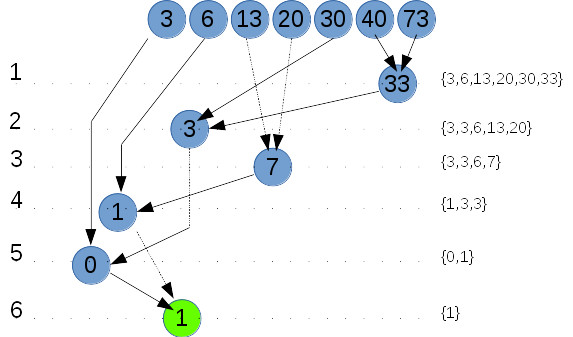
\includegraphics[width=\linewidth]
    {Biblio_PCmax_Rendu_exLDM_1_2m.jpg}
    \caption{Différentiation}
  	\end{subfigure}
\hfill% sinon, en fin de page, et pas sur la même ligne
% Backtracking à droite
	\begin{subfigure}[b]{0.45\linewidth}
    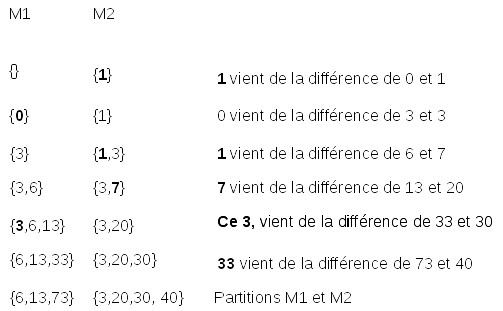
\includegraphics[width=\linewidth]
    {Biblio_PCmax_Rendu_exLDM_2_2m.jpg}
    \caption{Partitionnement (retour sur trace)}
  	\end{subfigure}
%CAPTION/FIGURE
  	\caption{LDM, avec $m=2$.}
  	\label{fig:LDM2M}
\end{figure}

\begin{example}
Soit $P=\{3,6,13,20,30,40,73\}$, l'ensemble des $P_j$.

40 et 73 sont les nombres les plus grands. On les remplace dans $P$ par $73 - 40 = 33$, pour donner $P=\{3,6,13,20,30,33\}$ et ainsi de suite.
La valeur restante est $P= \{1\}$, ce qui est le résultat de l'opération.
Par un retour sur trace, nous obtenons le partitionnement suivant:
$M_1 = \{ 6,13,73 \}$ et  $M_2 = \{ 3,20,30,40 \}$ (figure \ref{fig:LDM2M}).

\end{example}

\bigskip

\item cas de $m>2$, m sous-ensembles $M_1,M_2, \ldots, M_m $.

% PAS PERTINENT --------------------------------------------------
%Quelques rappels :
%
%Fonction densité :
%S'applique aux variables aléatoires continues (réelles), 
% pour lesquelles la probabilité ($\mathbb{P}$) d'appartenir à un domaine 
%($[a, b]$)  
%se calcule à l'aide d'une intégrale sur le domaine. 
%La fonction à intégrer ( $f(x)$ ) est la fonction de densité. 
%$\mathbb{P}(a \le X \le b) =  \int_{a}^b f(x)dx$.
%
%Condition de Lipschitz:
%Va déterminer la "douceur" d'une fonction. 
%Si une fonction répond à la condition de Lipschitz, 
%alors la pente maximale (en valeur absolue) du graphe représentant cette fonction 
%est inférieure à un nombre appelé Constante de Lipschitz.
%------------------------------------------------------------------
LDM effectue tout d'abord, une opération de préparation de l'instance du problème. Chaque élément de $P = \{ P_1, P_2, \ldots, P_n \}$ est converti en $m$-tuple. Les $m-1$ premiers composants sont vides, et le dernier (position m) est égal au nombre lui-même. Ainsi chaque $\underline{P_i} = \{P_{i 1}=0,P_{i 2}=0, \ldots, P_{i m}=\{P_i\} \}$

Puis, $n-1$ itérations des opérations suivantes sont effectuées:


Soit $d(\underline{P_i})$ la différence entre la valeur maximale et la valeur minimale des composants du sous-ensemble $\underline{P_i}$.

Extraction de $\underline{P_a}$ et $\underline{P_b}$ les deux m-tuples qui ont la plus grande différence $d(\underline{P_a})$ et $d(\underline{P_b})$. Ces deux solutions partielles, sont combinées pour former une nouvelle solution partielle $\underline{P_{ab}}$, en joignant le premier plus petit élément (ou l'élément vide) de $\underline{P_a}$ avec le premier élément le plus grand de $\underline{P_b}$, puis le deuxième élément le plus petit de $\underline{P_a}$ avec le deuxième élément le plus grand de $\underline{P_b}$ et ainsi de suite\ldots la nouvelle solution partielle $\underline{P_{ab}}$, remplace $\underline{P_a}$ et $\underline{P_b}$ dans l'instance.

Le résultat du partitionnement est donné après $n-1$ itérations.

%exemple
% ---------------------
\begin{example}

Soit $P=\{1,3,3,4,4,5,5,5\}$\\
nombre de machines $m=3$\\
\textbf{Création des m-tuples}:\\
\begin{multicols}{3}
$\underline{P_{1}} = \{,,1\}$\\
$\underline{P_{2}} = \{,,3\}$\\
$\underline{P_{3}} = \{,,3\}$\\
$\underline{P_{4}} = \{,,4\}$\\
$\underline{P_{5}} = \{,,4\}$\\
$\underline{P_{6}} = \{,,5\}$\\
$\underline{P_{7}} = \{,,5\}$\\
$\underline{P_{8}} = \{,,5\}$\\
\end{multicols}

\textbf{Itération 1}:\\
les tuples qui ont la différence la plus grande sont 
$\underline{P_{8}}$  et $\underline{P_{7}}$. 
on combine $\underline{P_{8}}$  et $\underline{P_{7}}$ pour créer un $\underline{P_{78}}$. Le premier plus petit élément de $\underline{P_{8}}$ (élément vide) est joint par le premier plus grand élément de $\underline{P_{8}}$ (5) pour donner  $\underline{P_{78}} = \{,5,5\}$. $d(\underline{P_{78}}) = 5-0 = 5$.\\
La nouvelle instance devient :\\
\begin{multicols}{3}
$\underline{P_{1}} = \{,,1\}$\\
$\underline{P_{2}} = \{,,3\}$\\
$\underline{P_{3}} = \{,,3\}$\\
$\underline{P_{4}} = \{,,4\}$\\
$\underline{P_{5}} = \{,,4\}$\\
$\underline{P_{6}} = \{,,5\}$\\
$\underline{P_{78}} = \{,5,5\}=5$\\
\end{multicols}

\textbf{Itération 2}:\\
On conbine $\underline{P_{6}}$ avec $\underline{P_{78}}$ pour donner $\underline{P_{678}} = \{5,5,5\}$. $d(\underline{P_{678}}) = 5-5 = 0$.\\
La nouvelle instance devient :\\
\begin{multicols}{3}
$\underline{P_{1}} = \{,,1\}$\\
$\underline{P_{2}} = \{,,3\}$\\
$\underline{P_{3}} = \{,,3\}$\\
$\underline{P_{4}} = \{,,4\}$\\
$\underline{P_{5}} = \{,,4\}$\\
$\underline{P_{678}} = \{5,5,5\}=0$\\
\end{multicols}

\textbf{Itération 3}:\\
les tuples qui ont la différence la plus grande sont 
$\underline{P_{5}}$  et $\underline{P_{4}}$. 
on les combine pour créer un $\underline{P_{45}}$. Le premier plus petit élément de $\underline{P_{5}}$ (élément vide) est joint par le premier plus grand élément de $\underline{P_{4}}$ (4) pour donner  $\underline{P_{45}} = \{,4,4\}$. $d(\underline{P_{45}}) = 4-0 = 4$.\\
La nouvelle instance devient :\\
\begin{multicols}{3}
$\underline{P_{1}} = \{,,1\}$\\
$\underline{P_{2}} = \{,,3\}$\\
$\underline{P_{3}} = \{,,3\}$\\
$\underline{P_{45}} = \{,4,4\}=4$\\
$\underline{P_{678}} = \{5,5,5\}=0$\\
\end{multicols}

\textbf{Itération 4}:\\
les tuples qui ont la différence la plus grande sont 
$\underline{P_{45}}$  et $\underline{P_{3}}$. 
on les combine pour créer un $\underline{P_{345}}$. Le premier plus petit élément de $\underline{P_{45}}$ (élément vide) est joint par le premier plus grand élément de $\underline{P_{3}}$ (3) pour donner  $\underline{P_{345}} = \{3,4,4\}$. $d(\underline{P_{345}}) = 4-3 = 1$.\\
La nouvelle instance devient :\\
\begin{multicols}{3}
$\underline{P_{1}} = \{,,1\}$\\
$\underline{P_{2}} = \{,,3\}$\\
$\underline{P_{345}} = \{3,4,4\}=1$\\
$\underline{P_{678}} = \{5,5,5\}=0$\\
\end{multicols}

\textbf{Itération 5}:\\
les tuples qui ont la différence la plus grande sont 
$\underline{P_{345}}$  et $\underline{P_{2}}$. 
on les combine pour créer un $\underline{P_{2345}}$. Le premier plus petit élément de $\underline{P_{345}}$ (3) est joint par le premier plus grand élément de $\underline{P_{2}}$ (3) pour donner  $\underline{P_{2345}} = \{(3,3),4,4\}$. La première association, vient d'être créée. elle a pour valeur 6. 
$d(\underline{P_{2345}}) = (3+3)-4 = 6-4=2$.\\
La nouvelle instance devient :\\
\begin{multicols}{2}
$\underline{P_{1}} = \{,,1\}$\\
$\underline{P_{2345}} = \{(3,3),4,4\}=2$\\
$\underline{P_{678}} = \{5,5,5\}=0$\\
\end{multicols}

\textbf{Itération 6}:\\
les tuples qui ont la différence la plus grande sont 
$\underline{P_{2345}}$  et $\underline{P_{1}}$. 
on les combine pour créer un $\underline{P_{2345}}$. Le premier plus petit élément de $\underline{P_{2345}}$ (4) est joint par le premier plus grand élément de $\underline{P_{2}}$ (1) pour donner  $\underline{P_{12345}} = \{(3,3),(1,4),4\}$.  
$d(\underline{P_{12345}}) = (3+3)-4 = 6-4=2$.\\
La nouvelle instance devient :\\
$\underline{P_{12345}} = \{(3,3),(1,4),4\}=2$\\
$\underline{P_{678}} = \{5,5,5\}=0$\\

\textbf{Itération 6}:\\
Reste à combiner $\underline{P_{12345}}$ et $\underline{P_{678}} = \{5,5,5\}=0$\\
Le premier plus petit élément de $\underline{P_{12345}}$ (4) est joint avec le premier plus grand de  $\underline{P_{678}}$ (5) et ainsi de suite... pour créer le résultat final \\
$\underline{P_{LDM}}= \{(3,3,5),(1,4,5),(4,5)\}$.\\
 
Nous avons donc un makespan $C_m^{LDM}(P) = 11 $ \\
Alors que $C_m^{\star}(P) = 10$ avec $\underline{P^{\star}}= \{(5,5),(1,4,5),(4,3,3)\}$.
\end{example}

\end{itemize}



% Complexité
% -------------------------------------------------------
\begin{theoreme}
\begin{flushleft}
\begin{tabular}{|p{8cm}p{6cm}|}
% TITRES (pas de titre)
\hline
% Ligne blanche
& \\
% Ligne Complexité
Complexité en temps \cite{michiels2003performance} :& $n^{- \Theta (log(n))}$
\\	% pas de ligne \hline
% Ligne blanche
& \\
% RATIO
Ratio \cite{michiels2003performance} &\\
% RATIO M= 2
pour $m=2$						& $\Gamma(LDM) = \dfrac{7}{6}$\\
pour $m\geq 3$					& $ \frac{4}{3}-\frac{1}{3 \cdot m} \leq
   									\Gamma(LDM) 						\leq 
   									\frac{4}{3}-\frac{1}{3 \cdot (m-1}$
\\
% Ligne blanche
& \\
\hline
\end{tabular}
%pas de legende
\end{flushleft}

\end{theoreme}


\subsubsection{d'autres algorithmes}
D'autres algorithme basés sur le partitionnement de nombres :

MPS, de Paletta et al \cite{paletta2007new}

SPS, de Chiaselotti \emph{et al.} \cite{chiaselotti2010minimizing}

 
\subsection{Autre}
% \subsubsection{algorithmes génétiques}
% \paragraph{algorithmes à réseaux de neurones}

\lp{Attention les algorithmes génétiques sont cosiédrés comme des méta
  heuristiques} \lp{Un algorithme génétique initialisé avec le
  résultat d'une heuristique performante donnera aussi un très bon
  résultat, tu ne peux donc pas dire qu'ils ne donnent pas de solution
  satisfaisantes. Par contre l'argument du temps tient bien. On a
  aussi aucune garantie sur le résultat puisque la recherche est
  aveugle. Mais il y a pas mal de travaux d'optimisation qui passent
  une couche de metaheuristique derrière une heuristique ou autre
  approx un pour voir s'il n'y aurait pas un meilleur résultat dans le
  voisinnage.}  D'autres pistes sont explorées pour répondre au
problème \problemGrahamP, comme l'algorithmique génétique,
l'utilisation de réseaux de neurones ou de méta-heuristiques. Mais il
s'avère que ces techniques sont très coûteuses en temps, et ne donnent
pas de solutions satisfaisantes. Ces techniques, complexes, sortent en
partie du cadre de cette bibliographie.

Min et al \cite{min1999genetic}

\section{Synthèse}


\subsection{Comparaisons}

Chaque étude du problème \problemGrahamP tente 
d'améliorer le ratio d'approximation, ainsi que le coût en temps requis 
pour obtenir cette solution approchée, 
soit en reprenant une piste déjà explorée afin de l'optimiser, 
soit en expérimentant d'autres méthodes. 
Les résultats théoriques attendus, définis et déterminés par
démonstrations, ne sont pas forcément cohérents avec les performances
réelles.\lp{Je ne comprends pas ce que tu veux dire par là}

\subsubsection{Théoriques}

% -------------------------------------------------------
% Tableau coupé en 2 car trop large !
% -------------------------------------------------------
% TABLEAU Comparatif RATIOS COÛTS EN TEMPS de chaque approche
% quand on les a !
% diagbox permet d'avoir une barre oblique pour les deux entrées
% \backslashbox{Instructions}{Donnée} & Simple & Multiple NE FONCTIONNE PAS
% on cadre à gauche le tableau pour avoir plus de place
% -------------------------------------------------------

Ce tableau est un comparatif des performances calculées et déterminées de chaque algorithme présenté. 

$n$ est le nombre de jobs à planifier.
$m$ est le nombre de machines parallèles identiques.
$k$ est un nombre d'itérations, soit  fixé via un paramètre de l'algorithme, ou le résultat d'une condition d'arrêt.
$\epsilon$ est un nombre positif ( e.g $\frac{1}{5}$ ) et désigne le ratio d'approximation d'un PTAS.

% 1/2
\begin{center}
\begin{tabular}{p{0.17\linewidth}
				p{0.16\linewidth}
				p{0.16\linewidth}
				p{0.16\linewidth}
				p{0.16\linewidth}
				p{0.16\linewidth}}

% ----------------------------------------------------
% TITRES
% ----------------------------------------------------
\hline
performance 						& 	
							LPT 	& 
							LPT-Rev &
							Slack 	&
							multifit& 
							combine  
%							listfit &
%							PA		&
%							PTAS	&
%							LDM  	\\
\\ \hline

% --------------------------
% LIGNE O()
% --------------------------
Complexité \newline (en temps) 		& 
							$O(n \cdot \log n) $ (*) &		% LPT
							$O(n \cdot \log n)$  (*) & 			% LPT-REV	
							$O(n \cdot \log n)$  (*) & 			% SLACK
							$O(n \log n + kn \log m)$& 		% MULTIFIT
							$O(n \log n + kn \log m)$		% COMBINE
													 
\\	\hline
% --------------------------
% LIGNE Ration
% --------------------------
Ratio \newline (pire des cas)		& 
							$\frac{4}{3} - \frac{1}{3m}$&		% LPT
							$\frac{4}{3} - \frac{1}{3(m-1)}$&	% LPT-REV
							/&								% SLACK (pas d'info)
							$1,220 + 2^{-k}$& 					% MULTIFIT
							$\frac{13}{12} + 2^{-k}$			% COMBINE
%---------------------------
\\
\hline
\end{tabular}
Comparaison des performances des algorithmes présentés. tableau 1/2.

(*) $+ (n \cdot \log m)$ si on prend en compte le tri des jobs au préalable.
\end{center}

% 2/2
\begin{center}
\begin{tabular}{p{0.17\linewidth}
				p{0.16\linewidth}
				p{0.16\linewidth}
				p{0.16\linewidth}
				p{0.32\linewidth}}


% ----------------------------------------------------
% TITRES
% ----------------------------------------------------
\hline
performance 						& 	
							listfit &
							PA		&
							PTAS	&
							LDM  	
\\ \hline

% --------------------------
% LIGNE O()
% --------------------------
Complexité \newline (en temps) & 
							$O(n^2 \log(n) + k \cdot n^2 \log(m))$&	% LISTFIT
							/& 		% PA (pas d'infos)
							$ O(( \frac{n}{\epsilon})^\frac{1}{\epsilon ^ 2})$&
					 		$n^{- \Theta (log(n))}$% LDM
						 
\\	\hline
% --------------------------
% LIGNE Ration
% --------------------------
Ratio \newline (pire des cas)		& 
							$\dfrac{13}{12} + 2^{-k}$&		% LISTFIT
							/&								% PA (pas d'info)
							$1 + \epsilon$	&				%PTAS
							compris entre \newline						% LDM
								$\frac{4}{3}-\frac{1}{3 \cdot m}$ et	% LDM
								\newline 								% LDM
								$\frac{4}{3}-\frac{1}{3 \cdot (m-1}$	%LDM

%---------------------------
\\
\hline
\end{tabular}
Comparaison des performances des algorithmes présentés. tableau 2/2.
\end{center}

LPT rule et LPT-REV présentent un ratio d'approximation qui s'approche du pire cas lorsque le nombre de machines augmente. Multifit, Combine et Listfit se suivent dans leurs performances (ListFit est plus coûteux en temps). Concernant le PTAS, plus $\epsilon$ est petit (ratio tend vers $1$)  plus l'algorithme se rapproche de la solution optimale, mais plus il pèse dans la complexité en temps (exponentiel en $\epsilon$).


\subsubsection{Expérimentales}

\begin{figure}
\centering
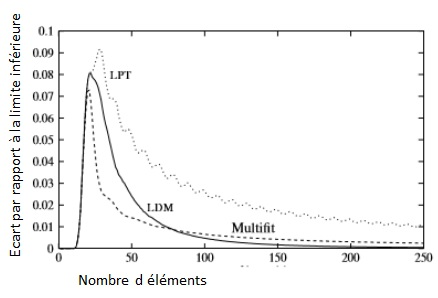
\includegraphics[width=10cm,height=6.80cm]
{Biblio_PCmax_Rendu_CompborneInf_LPT_LDM_MULTIFIT.jpg}
\caption{Écarts moyen de LPT, LDM, Multifit, par rapport à la borne inférieure de  10 000 instances créées pour chaque nombre n d'éléments et m=10 machines.}
\label{comparaison:LPTLDMMFBorneInf}
\end{figure}

En général, LPT donne des performances pratiques bien meilleures que les ratios théoriques attendus \cite{della2018longest}, surtout dans les instances à nombre élevé de jobs. 

Michiels \emph{et al.} \citep{michiels2003performance} étudient les performances des trois algorithmes phares (LPT, LDM, et Multifits), pour un nombre m=10 machines, et en fonction du nombre n d'éléments. Pour chaque n, 10 000 instances sont créées, à l'aide de nombres (temps des jobs) uniformément répartis (instances uniformes) dans l'intervalle [0,1]. La figure \ref{comparaison:LPTLDMMFBorneInf} représente l'écart moyen de chaque algorithme 
par rapport à la borne inférieure (théorème \ref{theoreme:borneMini}). 
LPT est le moins performant, et Multifit supplante LDM à partir de $n=79$ éléments. Néanmoins, cette étude se base sur des éléments uniformément répartis, condition où LDM est très performant.

Slack \ref{algo:SLACK}, qui n'est autre que LPT amélioré d'une heuristique, et accompagné d'une recherche locale devient globalement plus performant que LDM \cite{della2018longest}.

Gupta \emph{et al.} prouvent que les performances de ListFit \ref{algo:LISTFIT} sont supérieures à LPT, Multifit et Combine.Ceux-ci sont comparés \cite{gupta2001listfit} \cite{lee1988multiprocessor} suivant des indices, en mettant de côté le nombre  k nécessaires à l’Achèvement des algorithmes. Behera et al \cite{behera2012comparison} comparent dans une étude le coût processeur de chaque heuristique, Qui indique que Listfit est très gourmand.


\begin{center}
\begin{tabular}{p{0.19\linewidth}
				p{0.19\linewidth}
				p{0.19\linewidth}
				p{0.19\linewidth}
				p{0.19\linewidth}}
% ----------------------------------------------------
% TITRES
% ----------------------------------------------------
\hline
n		&	m	&	Multifit	&	Combine	&	Listfit

\\ \hline \\							
% --------------------------
% LIGNE des 100
% --------------------------
100		&	2	&	20			&	22		&	1767 	\\
		&	3	&	24			&	32		&	1968	\\
		&	6	&	20			&	44		&	3293	\\
		&	8	&	20			&	56		&	3755		
\\ \hline \\							
200		&	2	&	44			&	66		&	7269 	\\
		&	3	&	44			&	66		&	8153	\\
		&	6	&	64			&	132		&	13695	\\
		&	8	&	64			&	154		&	15422		
\\ \hline \\							
300		&	2	&	88			&	120		&	15663	\\
		&	3	&	112			&	132		&	17671	\\
		&	6	&	108			&	176		&	25673	\\
		&	8	&	132			&	198		&	29558		
% FIN ----------------------------------------
\\ \hline \\
\end{tabular}
Comparaison des temps moyens pour Multifit, Combine et Listfit 
\newline (en $10^{-6} secondes$)
\end{center}


\subsection{De la recherche d'informations}
Il a été très difficile, voire impossible de trouver plus d'informations sur les performances  
de PA \ref{algo:PA} (résolution du problème \problemGrahamP par programmation linéaire), 
du PTAS dual-approximation \ref{algo:PTASDual1_5}   \ref{algo:PTASDual1_6}. En effet, Il aurait été intéressant d'avoir un aperçut de la complexité en temps de PA (Programmation linéaire + Branch\&Bound) et l'algorithme générique (non optimisé pour $\epsilon = \frac{1}{5}$ et $\epsilon = \frac{1}{6}$) du PTAS dual-approximation en programmation dynamique.

\section{Conclusion}

Dans cette bibliographie non-exhaustive, nous venons de voir différentes approches qui tentent de répondre au problème d'ordonnancement \problemGrahamP, 
soit directement, soit indirectement via des problèmes similaires, 
tels que le Bin-Packing ou le partitionnement de nombres.
Chacune de ces méthodes a ses avantages et ses défauts. Soit leur complexité en temps est intéressante, mais leur ratio d'approximation est élevé, ou inversement, le résultat obtenu est très proche de l'optimal, au détriment d'un coût élevé en temps.

Il sera intéressant de définir un protocole expérimental afin de créer 
un spectre d'instances du problème plus complet, pour produire 
une comparaison d'un ensemble d'heuristiques.

Et enfin, ces résultats pourrons être utilisés pour d'autres problèmes d'ordonnancements (contraintes, processeurs/machines hétérogènes).

\section{remerciements}
Laurent Philippe
Louis-Claude Canon
Julien Bernard
Professeurs et personnel du CTU 


\medskip


\bibliographystyle{plain}				% NE PAS ENLEVER !!!!!!!!!!
\bibliography{Bibliographie}			% Utilise Bibliographie.bib








\end{document}
